\section{Ứng dụng kết nối tới cơ sở dữ liệu}
\subsection{Tổng quan công nghệ}
\textbf{Về Front-end}:
\begin{itemize}
    \item [--] Công nghệ sử dụng: Vite và React.
    \item [--] Giao diện người dùng được xây dựng bằng React, kết hợp với Vite để tối ưu hóa quá trình phát triển và đóng gói. React được sử dụng để tạo các thành phần giao diện động, giúp hiển thị dữ liệu nhân sự và cung cấp các chức năng quản lý như thêm mới, chỉnh sửa, và xóa thông tin nhân viên. Giao diện người dùng giao tiếp với backend thông qua API.
\end{itemize}

\textbf{Về Back-end}:
\begin{itemize}
    \item [--] Công nghệ sử dụng: Node.js và Express.js.
    \item [--] Backend đóng vai trò xử lý logic nghiệp vụ và cung cấp API RESTful để phục vụ yêu cầu từ frontend. Express.js giúp tổ chức các endpoint một cách rõ ràng và dễ mở rộng. 
\end{itemize}

\textbf{Về Database}:
\begin{itemize}
    \item [--] Công nghệ sử dụng: MySQL
    \item [--] Dữ liệu nhân sự được lưu trữ trong MySQL, sử dụng các bảng để quản lý thông tin nhân viên, phòng ban, và các mối quan hệ liên quan.
\end{itemize}

\textbf{Giao tiếp giữa các phần}:
\begin{itemize}
    \item [--] Frontend và backend giao tiếp qua HTTP/HTTPS thông qua các API RESTful. Dữ liệu được truyền dưới dạng JSON.
    \item [--] Backend sử dụng thư viện MySQL2 kết nối MySQL để truy xuất và xử lý dữ liệu, sau đó trả về kết quả cho frontend.
\end{itemize}

\newpage
\subsection{Khai báo kết nối đến MySQL}
Kết nối đến MySQL được khởi tạo ở file \texttt{database.js} như sau:
\begin{minted}{javascript}
import msyql from 'mysql2/promise'
import { configDotenv } from 'dotenv'
configDotenv()

const connection_info = {
    host: process.env.MYSQL_HOST,
    user: process.env.MYSQL_USER,
    password: process.env.MYSQL_PASSWORD,
    database: process.env.MYSQL_DATABASE,
    rowsAsArray: true,
}

export async function ReadQuery(sql, param) {
    let result = '';
    let success = true
    try {
        const connection = await msyql.createConnection(connection_info)
        result = await connection.execute(sql, param);
    } catch (error) {
        console.log(error.message)
        success = false;
    }
    return result[0];
}
\end{minted}

Để thực hiện một câu lệnh SQL, người dùng cần tạo một API mới trong file \texttt{api.js} và tạo một đường dẫn đến nó trong file \texttt{index.js}. Ví dụ: API để đọc toàn bộ dữ liệu từ bảng NhanVien:
\begin{minted}{javascript}
    // ################### api.js #####################
    export const getNhanVien = async () => {
        const rows = await ReadQuery('SELECT * FROM NhanVien');
        return rows;
    };
    // ################### api.js #####################

    // ################### index.js #####################
    app.get('/api/nhanvien', async function (req, res) {
        const nhanvien = await getNhanVien();
        res.send({nhanvien})
    })
    // ################### index.js #####################
\end{minted}

\newpage
\subsection{Các màn hình demo}
\subsubsection{Màn hình 1}
\textbf{Bao gồm các màn hình}: Xem thông tin nhân viên, thêm nhân viên và sửa nhân viên. Có tính năng phân trang và xóa một nhân viên.

Màn hình hiển thị bảng thông tin tất cả các nhân viên trong công ty
\begin{figure}[H]
    \centering
    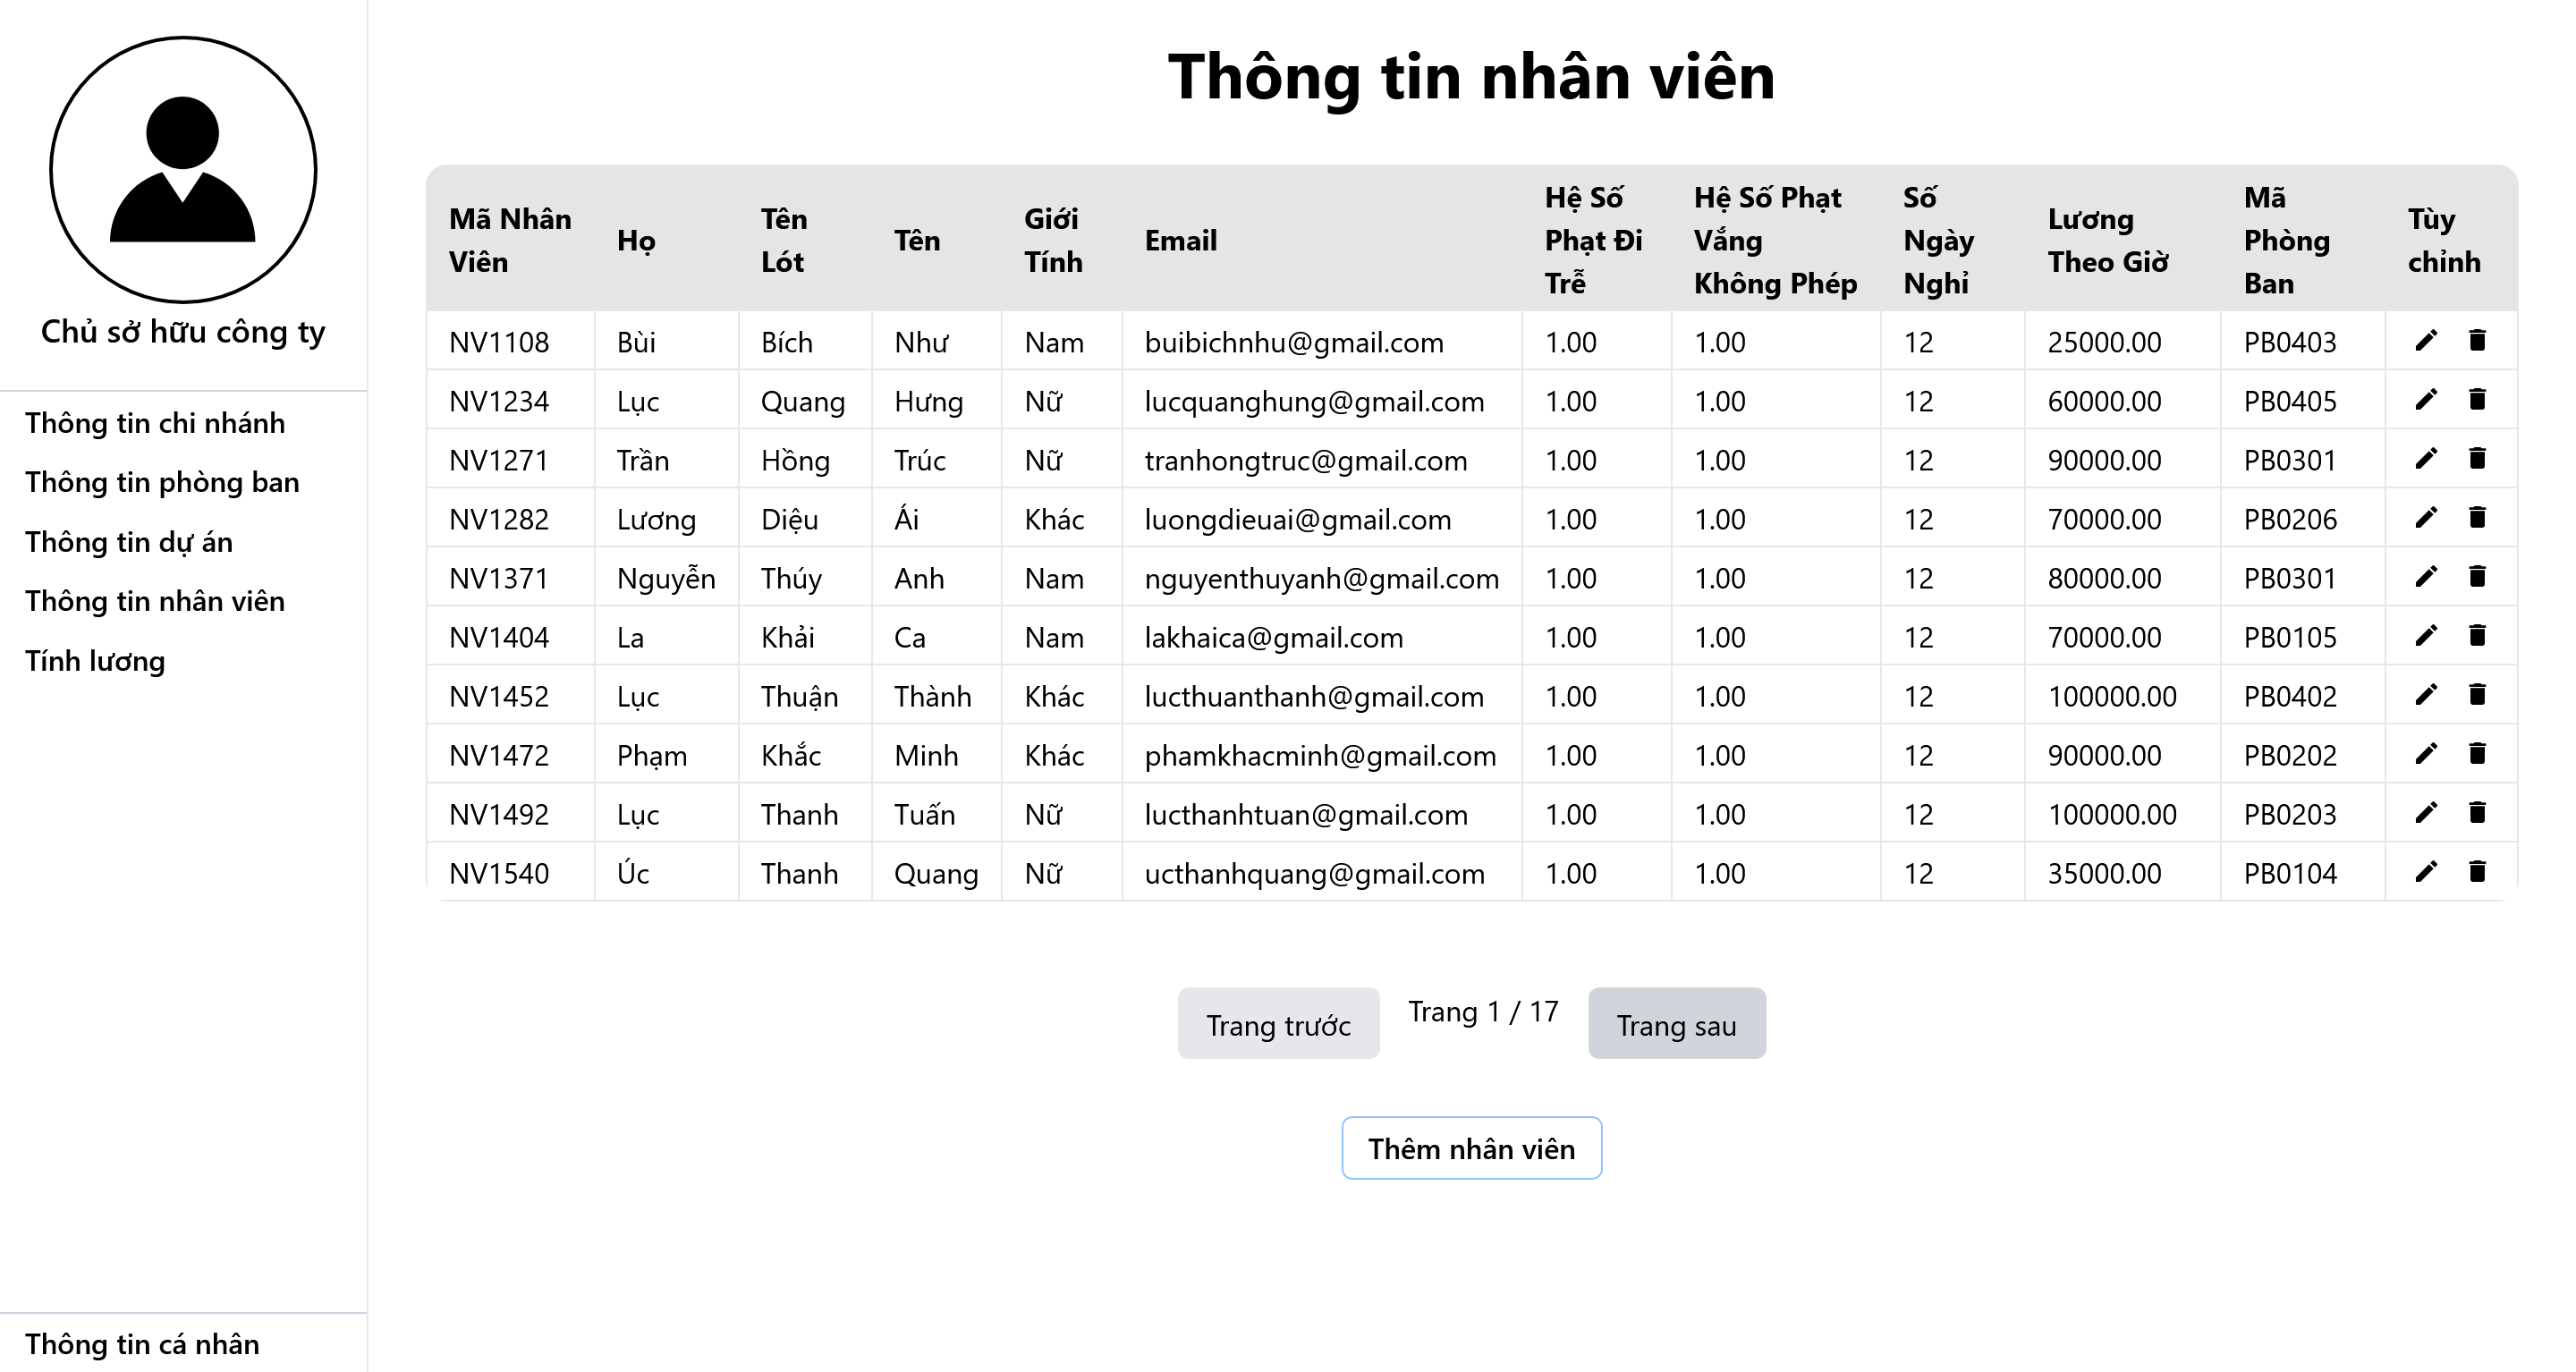
\includegraphics[width=0.75\linewidth]{content/images/ManHinh_1_1.png}
    \caption{Hiển thị thông tin bảng NhanVien, được sắp xếp mặc định theo mã nhân viên theo thứ tự a-z}
    \label{fig:ManHinh_1_1}
\end{figure}

Màn hình hiển thị trang thêm nhân viên, nơi để người dùng thêm một nhân viên mới vào công ty.
\begin{itemize}
    \item [--] Màn hình có những input field cho người dùng nhập thông tin nhân viên mới vào.
    \item [--] Nút 'Quay lại' để quay về trang hiển thị bảng thông tin toàn bộ nhân viên
    \item [--] Nút 'Thêm nhân viên' dùng để thêm nhân viên, màn hình sẽ thông báo thành công và cập nhật lên cơ sở dữ liệu thông tin về nhân viên mới nếu người dùng nhập đầy đủ thông tin, đúng định dạng và không trùng mã nhân viên, nếu không màn hình sẽ thông báo lỗi và không thực hiện việc thêm nhân viên.
    \item [--] Nút 'Nhập lại' dùng để xóa toàn bộ những thông tin trong các input field.
\end{itemize}

\begin{figure}[H]
    \centering
    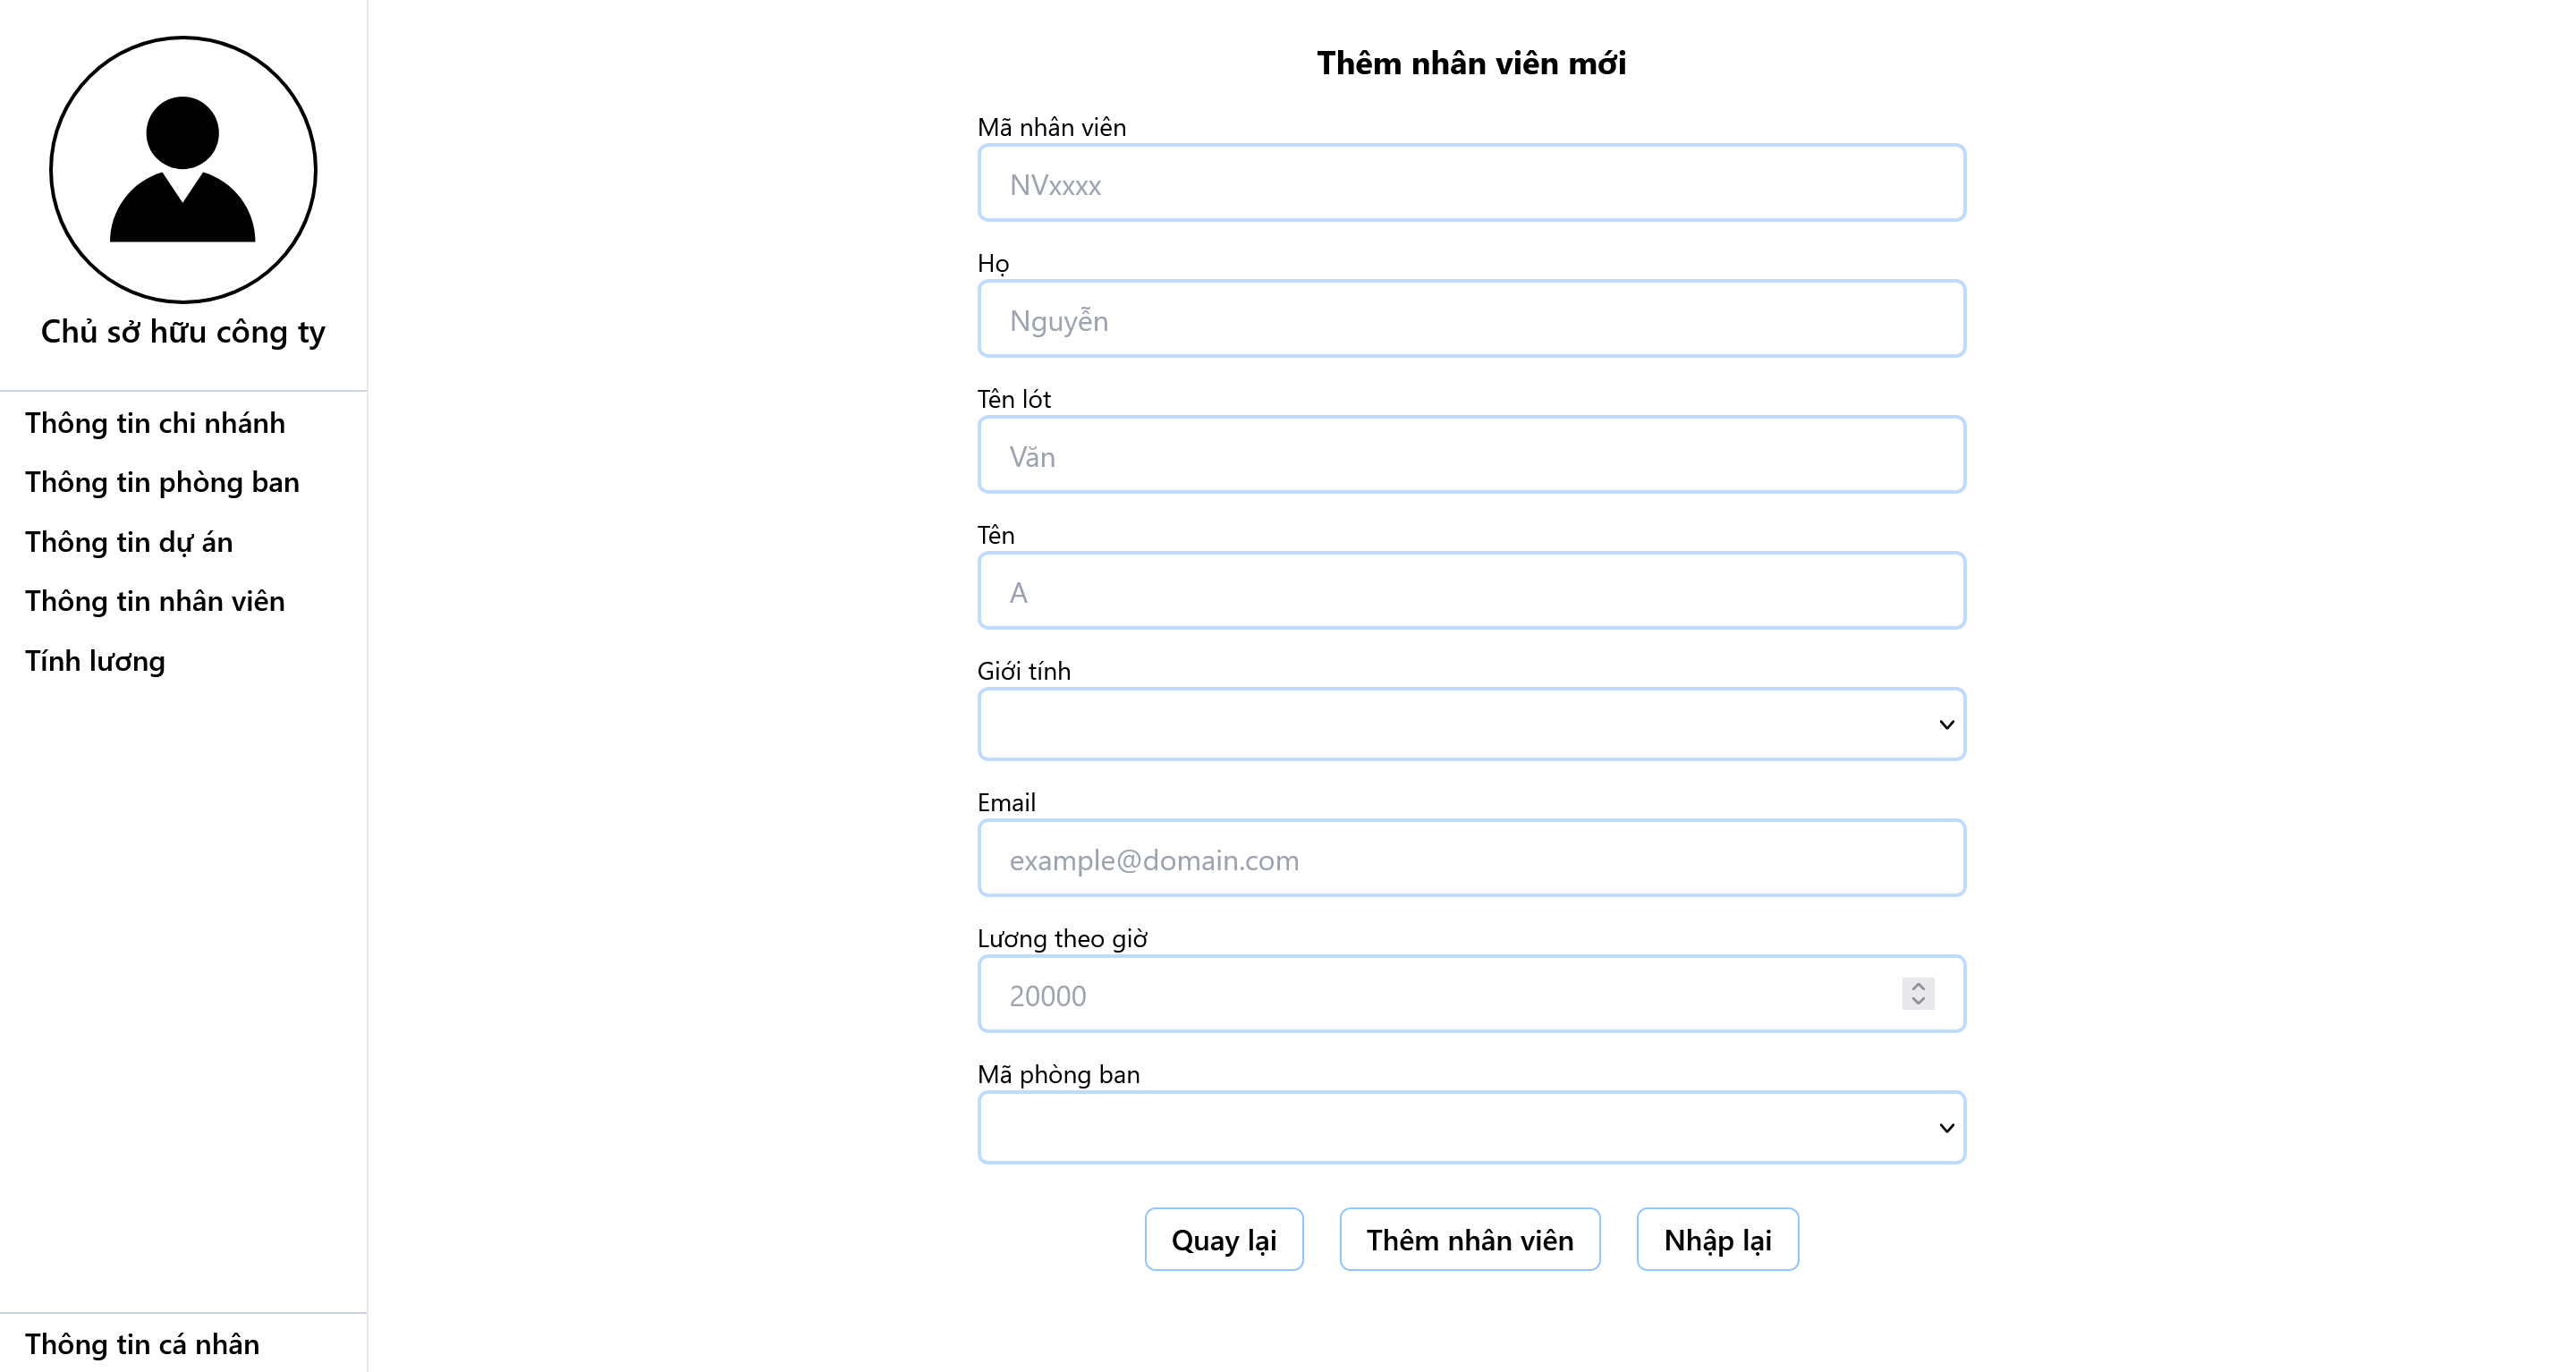
\includegraphics[width=0.75\linewidth]{content/images/ManHinh_1_a.png}
    \caption{Màn hình hiển thị trang thêm nhân viên}
    \label{fig:ManHinh_1_a}
\end{figure}

Khi có lỗi xảy ra, như lỗi sai định dạng thông tin của nhân viên, màn hình sẽ thông báo lỗi cho người dùng
\begin{figure}[H]
    \centering
    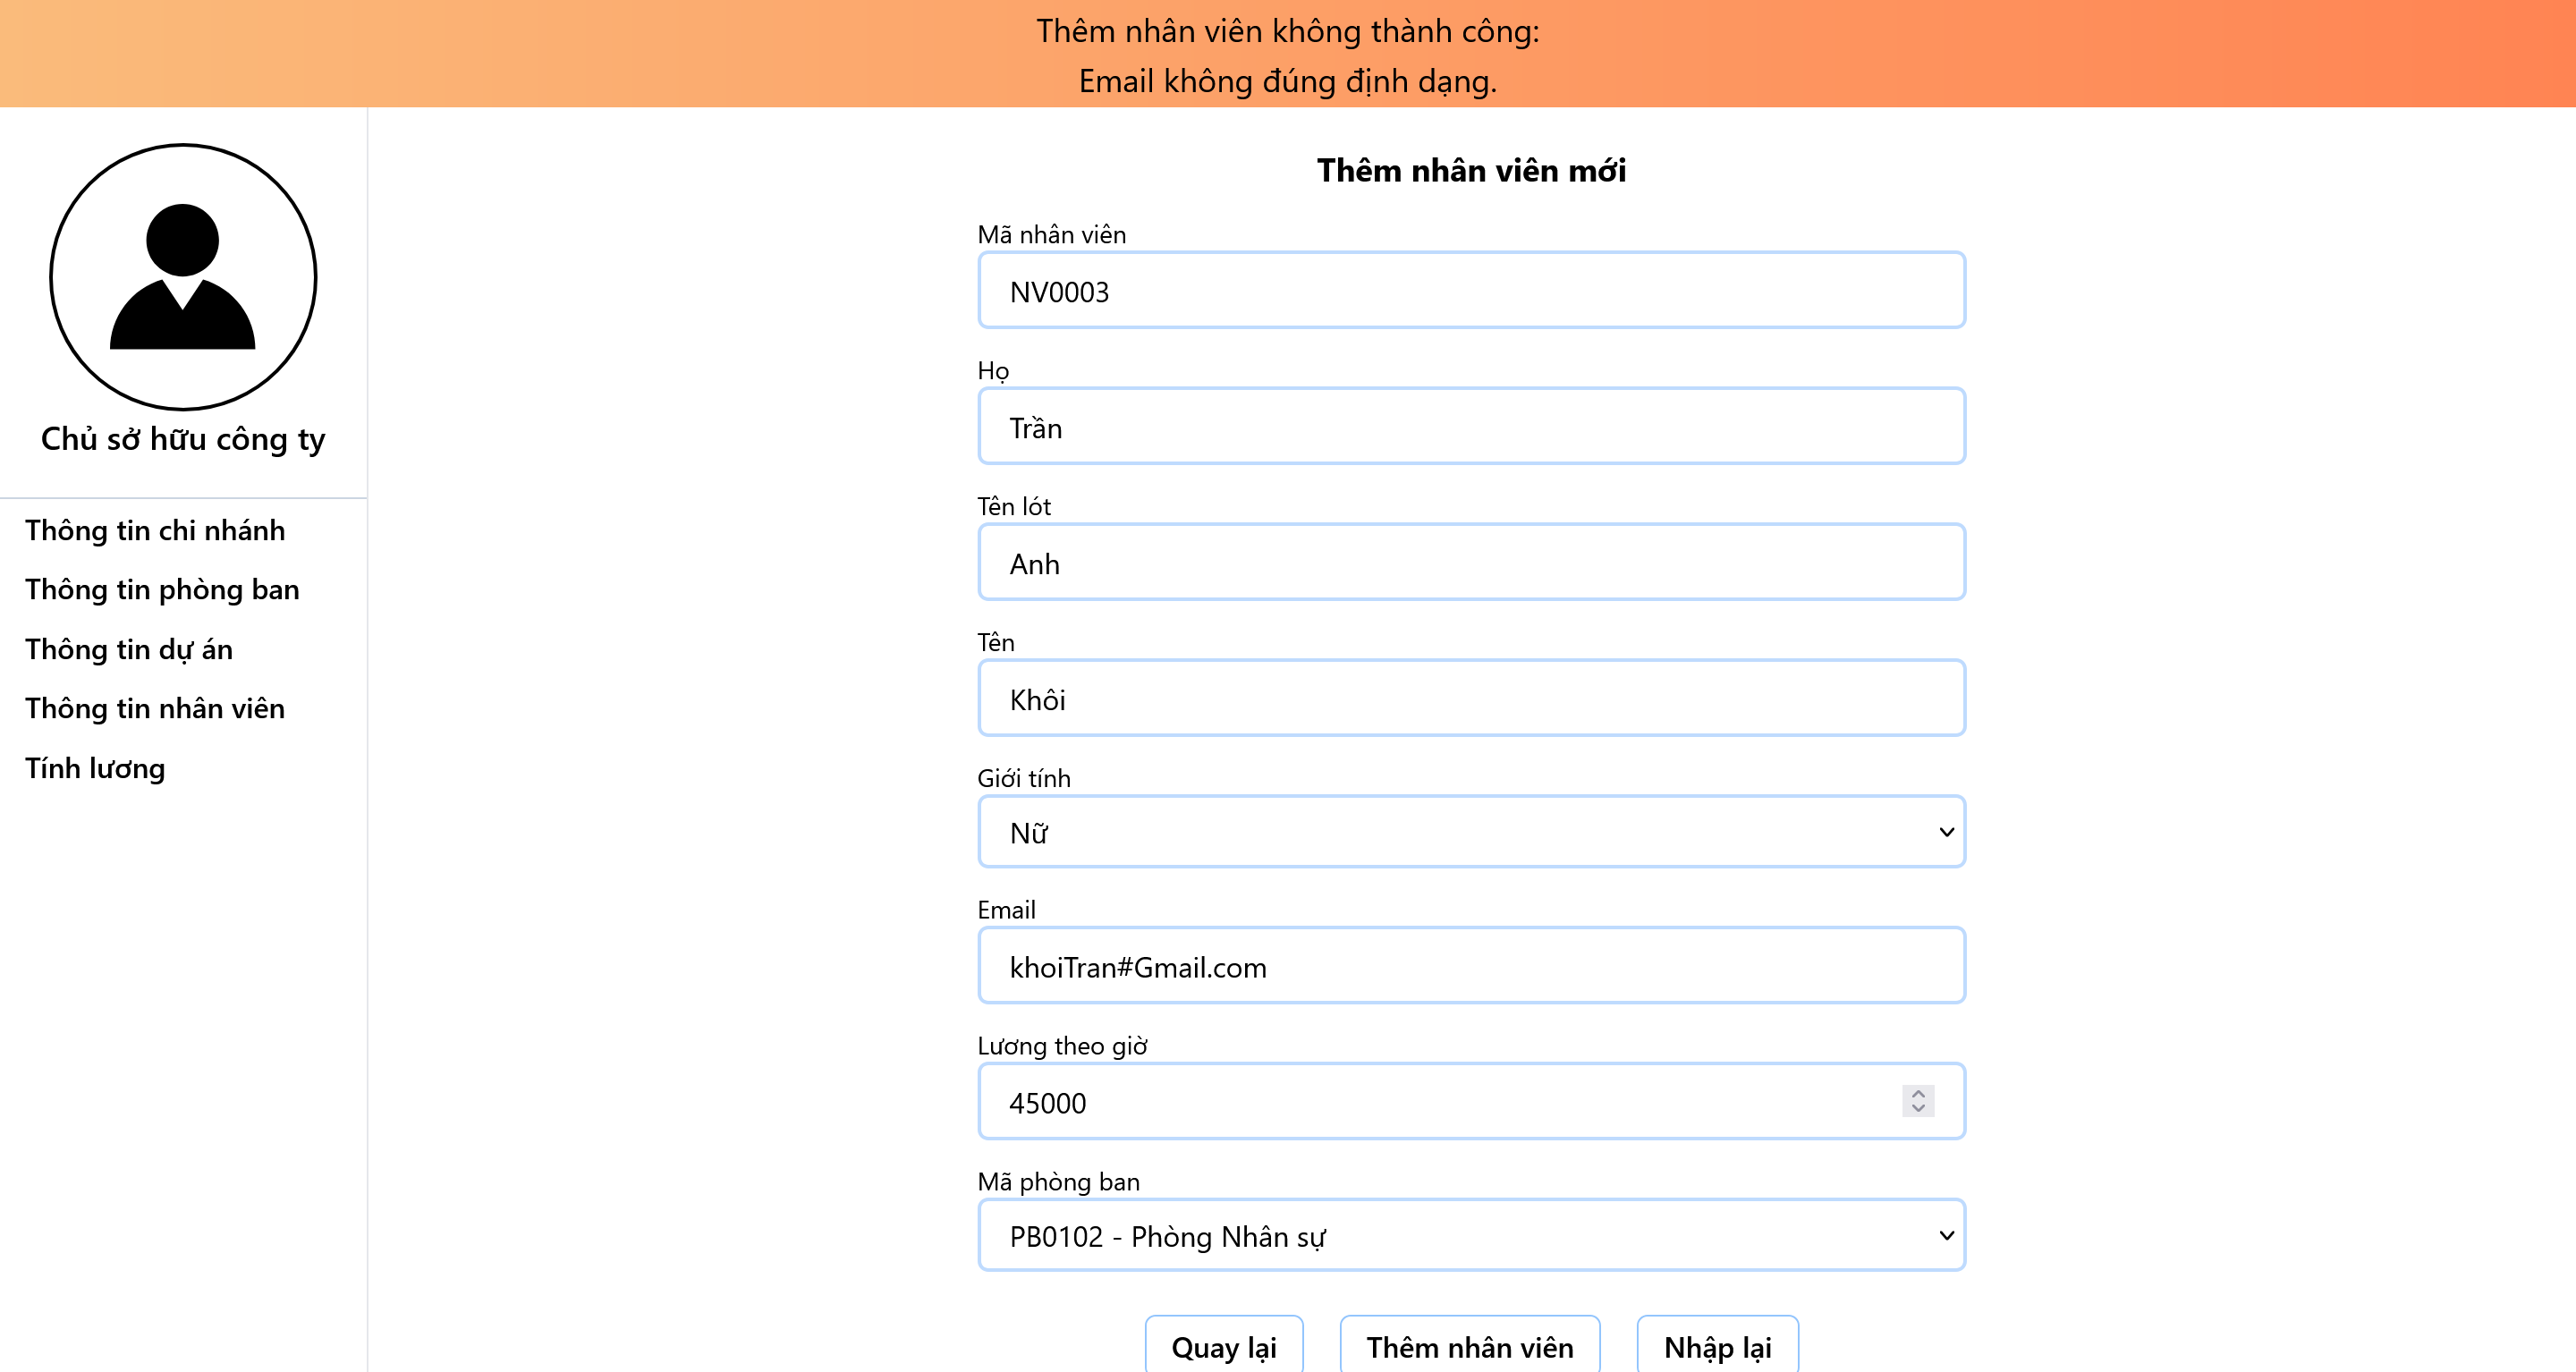
\includegraphics[width=0.75\linewidth]{content/images/ManHinh_1_b.png}
    \caption{Màn hình thêm nhân viên - thất bại do sai định dạng email}
    \label{fig:ManHinh_1_b}
\end{figure}

Khi đã nhập đúng định dạng và đầy đủ thông tin, khi nhấn nút thêm nhân viên, màn hình sẽ thông báo thành công và cập nhật lên cơ sở dữ liệu
\begin{figure}[H]
    \centering
    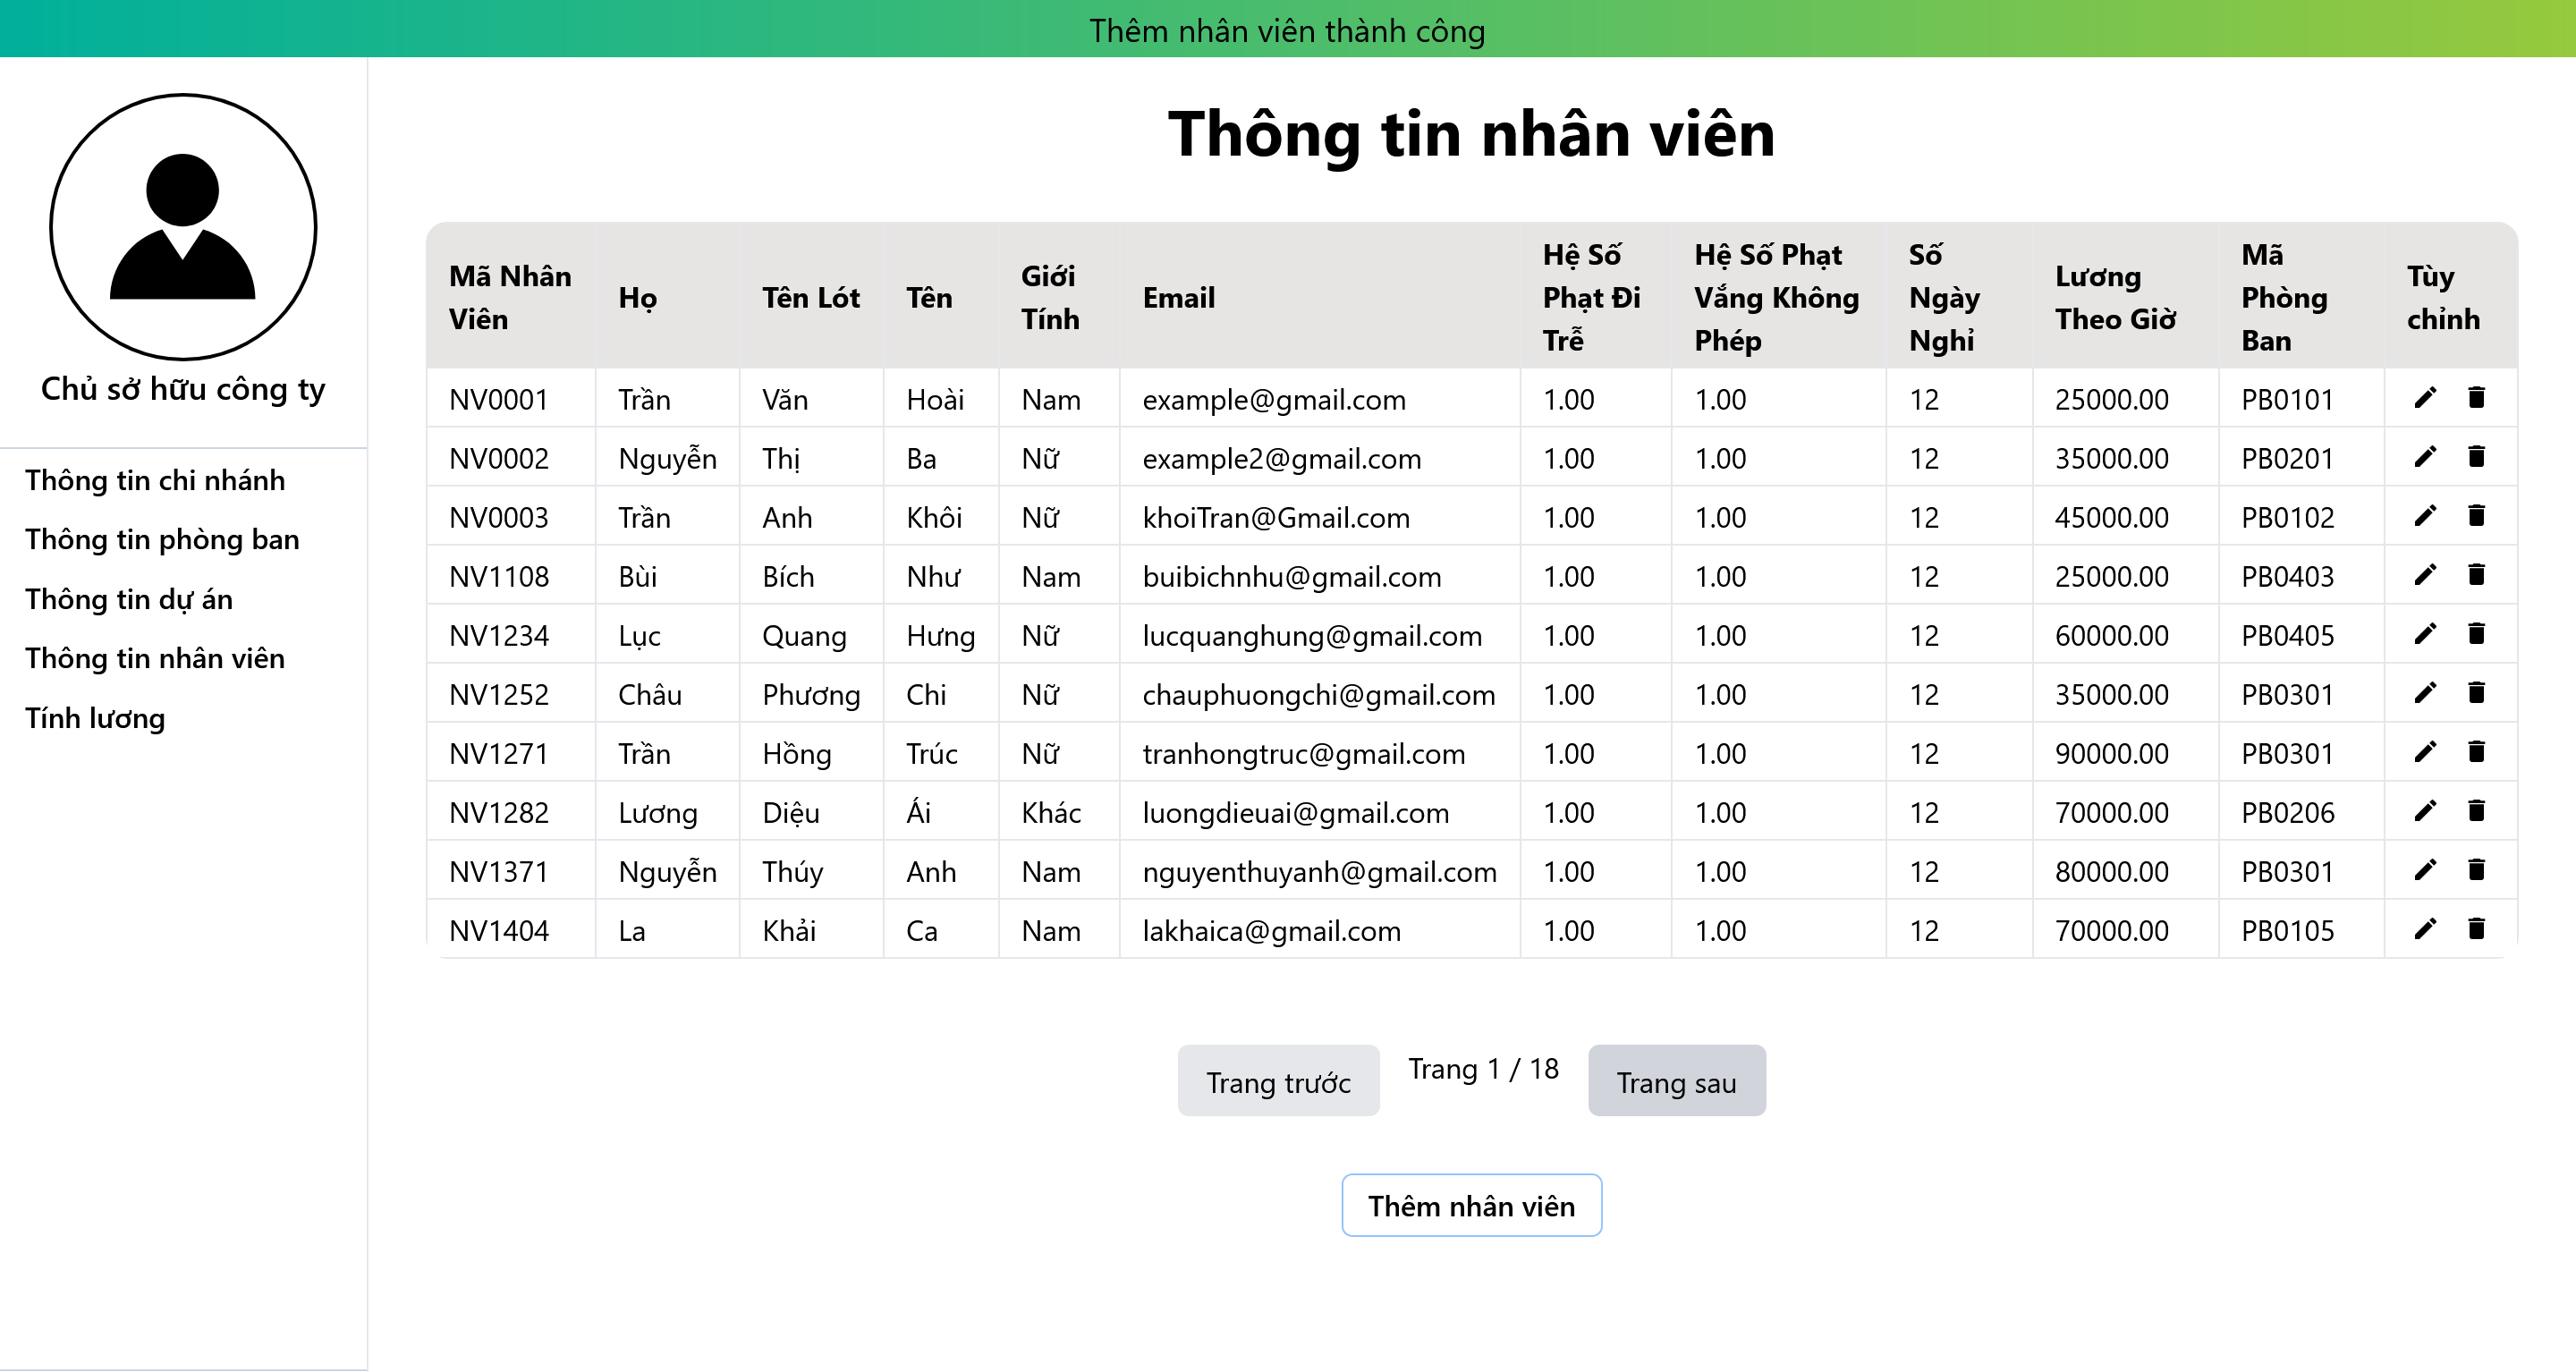
\includegraphics[width=0.75\linewidth]{content/images/ManHinh_1_c.png}
    \caption{Màn hình thêm nhân viên - thành công}
    \label{fig:ManHinh_1_c}
\end{figure}


Tra cứu thông tin nhân viên vừa được thêm mới trực tiếp trên cơ sở dữ liệu để kiểm chứng hoạt động
\begin{figure}[H]
    \centering
    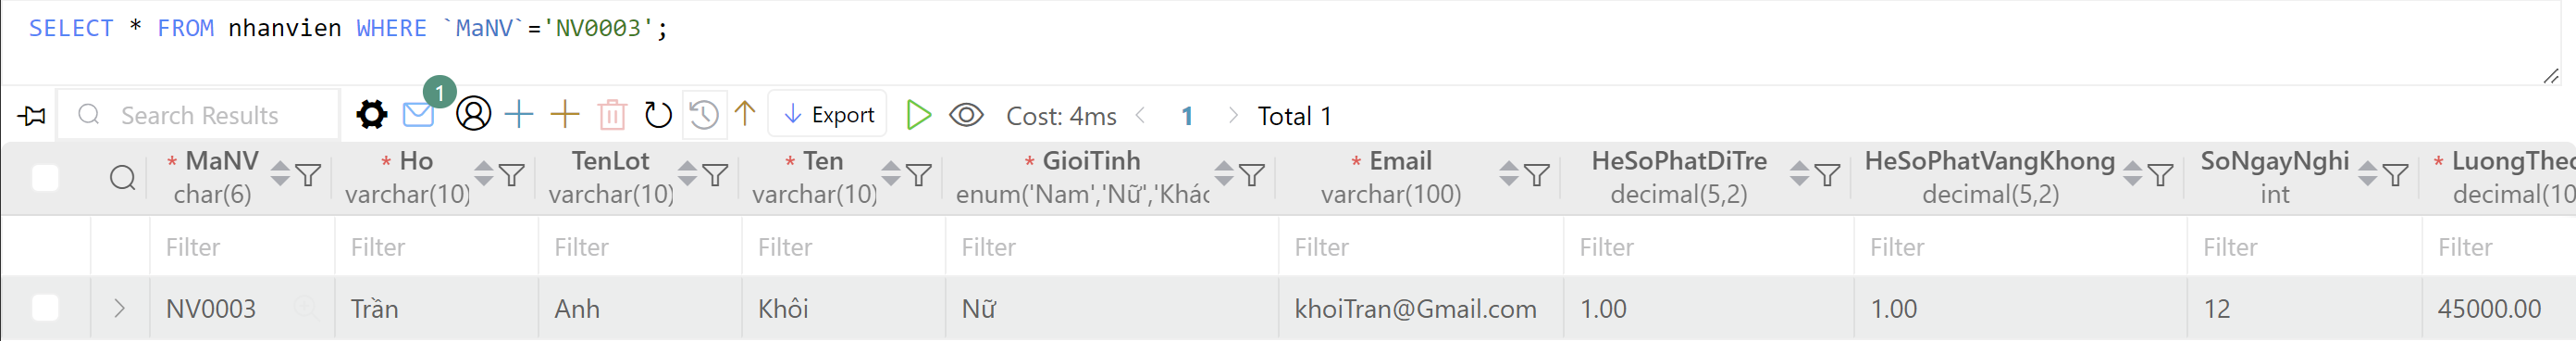
\includegraphics[width=0.75\linewidth]{content/images/ManHinh_1_d.png}
    \caption{Tra cứu thành công, nhân viên vừa được thêm ở trang web đã được cập nhật bên phía back-end}
    \label{fig:ManHinh_1_d}
\end{figure}

Để chỉnh sửa thông tin của một nhân viên cụ thể, người dùng phải tìm đến hàng chứa thông tin của nhân viên mình muốn cập nhật và click vào icon cây bút ở trong hàng đó, khi đó màn hình chỉnh sửa thông tin sẽ được hiện ra.

Màn hình chỉnh sửa thông tin nhân viên
\begin{itemize}
    \item [--] Màn hình có những input field cho người dùng nhập thông tin vào với những placeholder là thông tin hiện tại của nhân viên đó.
    \item [--] Người dùng có thể nhập vào bất cứ field nào mà mình muốn cập nhật, không bắt buộc phải nhập hết toàn bộ.
    \item [--] Nút 'Cập nhật' dùng để tiến hành cập nhật thông tin nhân viên, màn hình sẽ thông báo thành công và cập nhật lên cơ sở dữ liệu nếu người dùng nhập đúng định dạng các field muốn cập nhật, nếu không màn hình sẽ thông báo lỗi và không thực hiện việc cập nhật thông tin nhân viên.
    \item [--] Nút 'Quay lại' để quay về trang hiển thị bảng thông tin toàn bộ nhân viên
\end{itemize}
\begin{figure}[H]
    \centering
    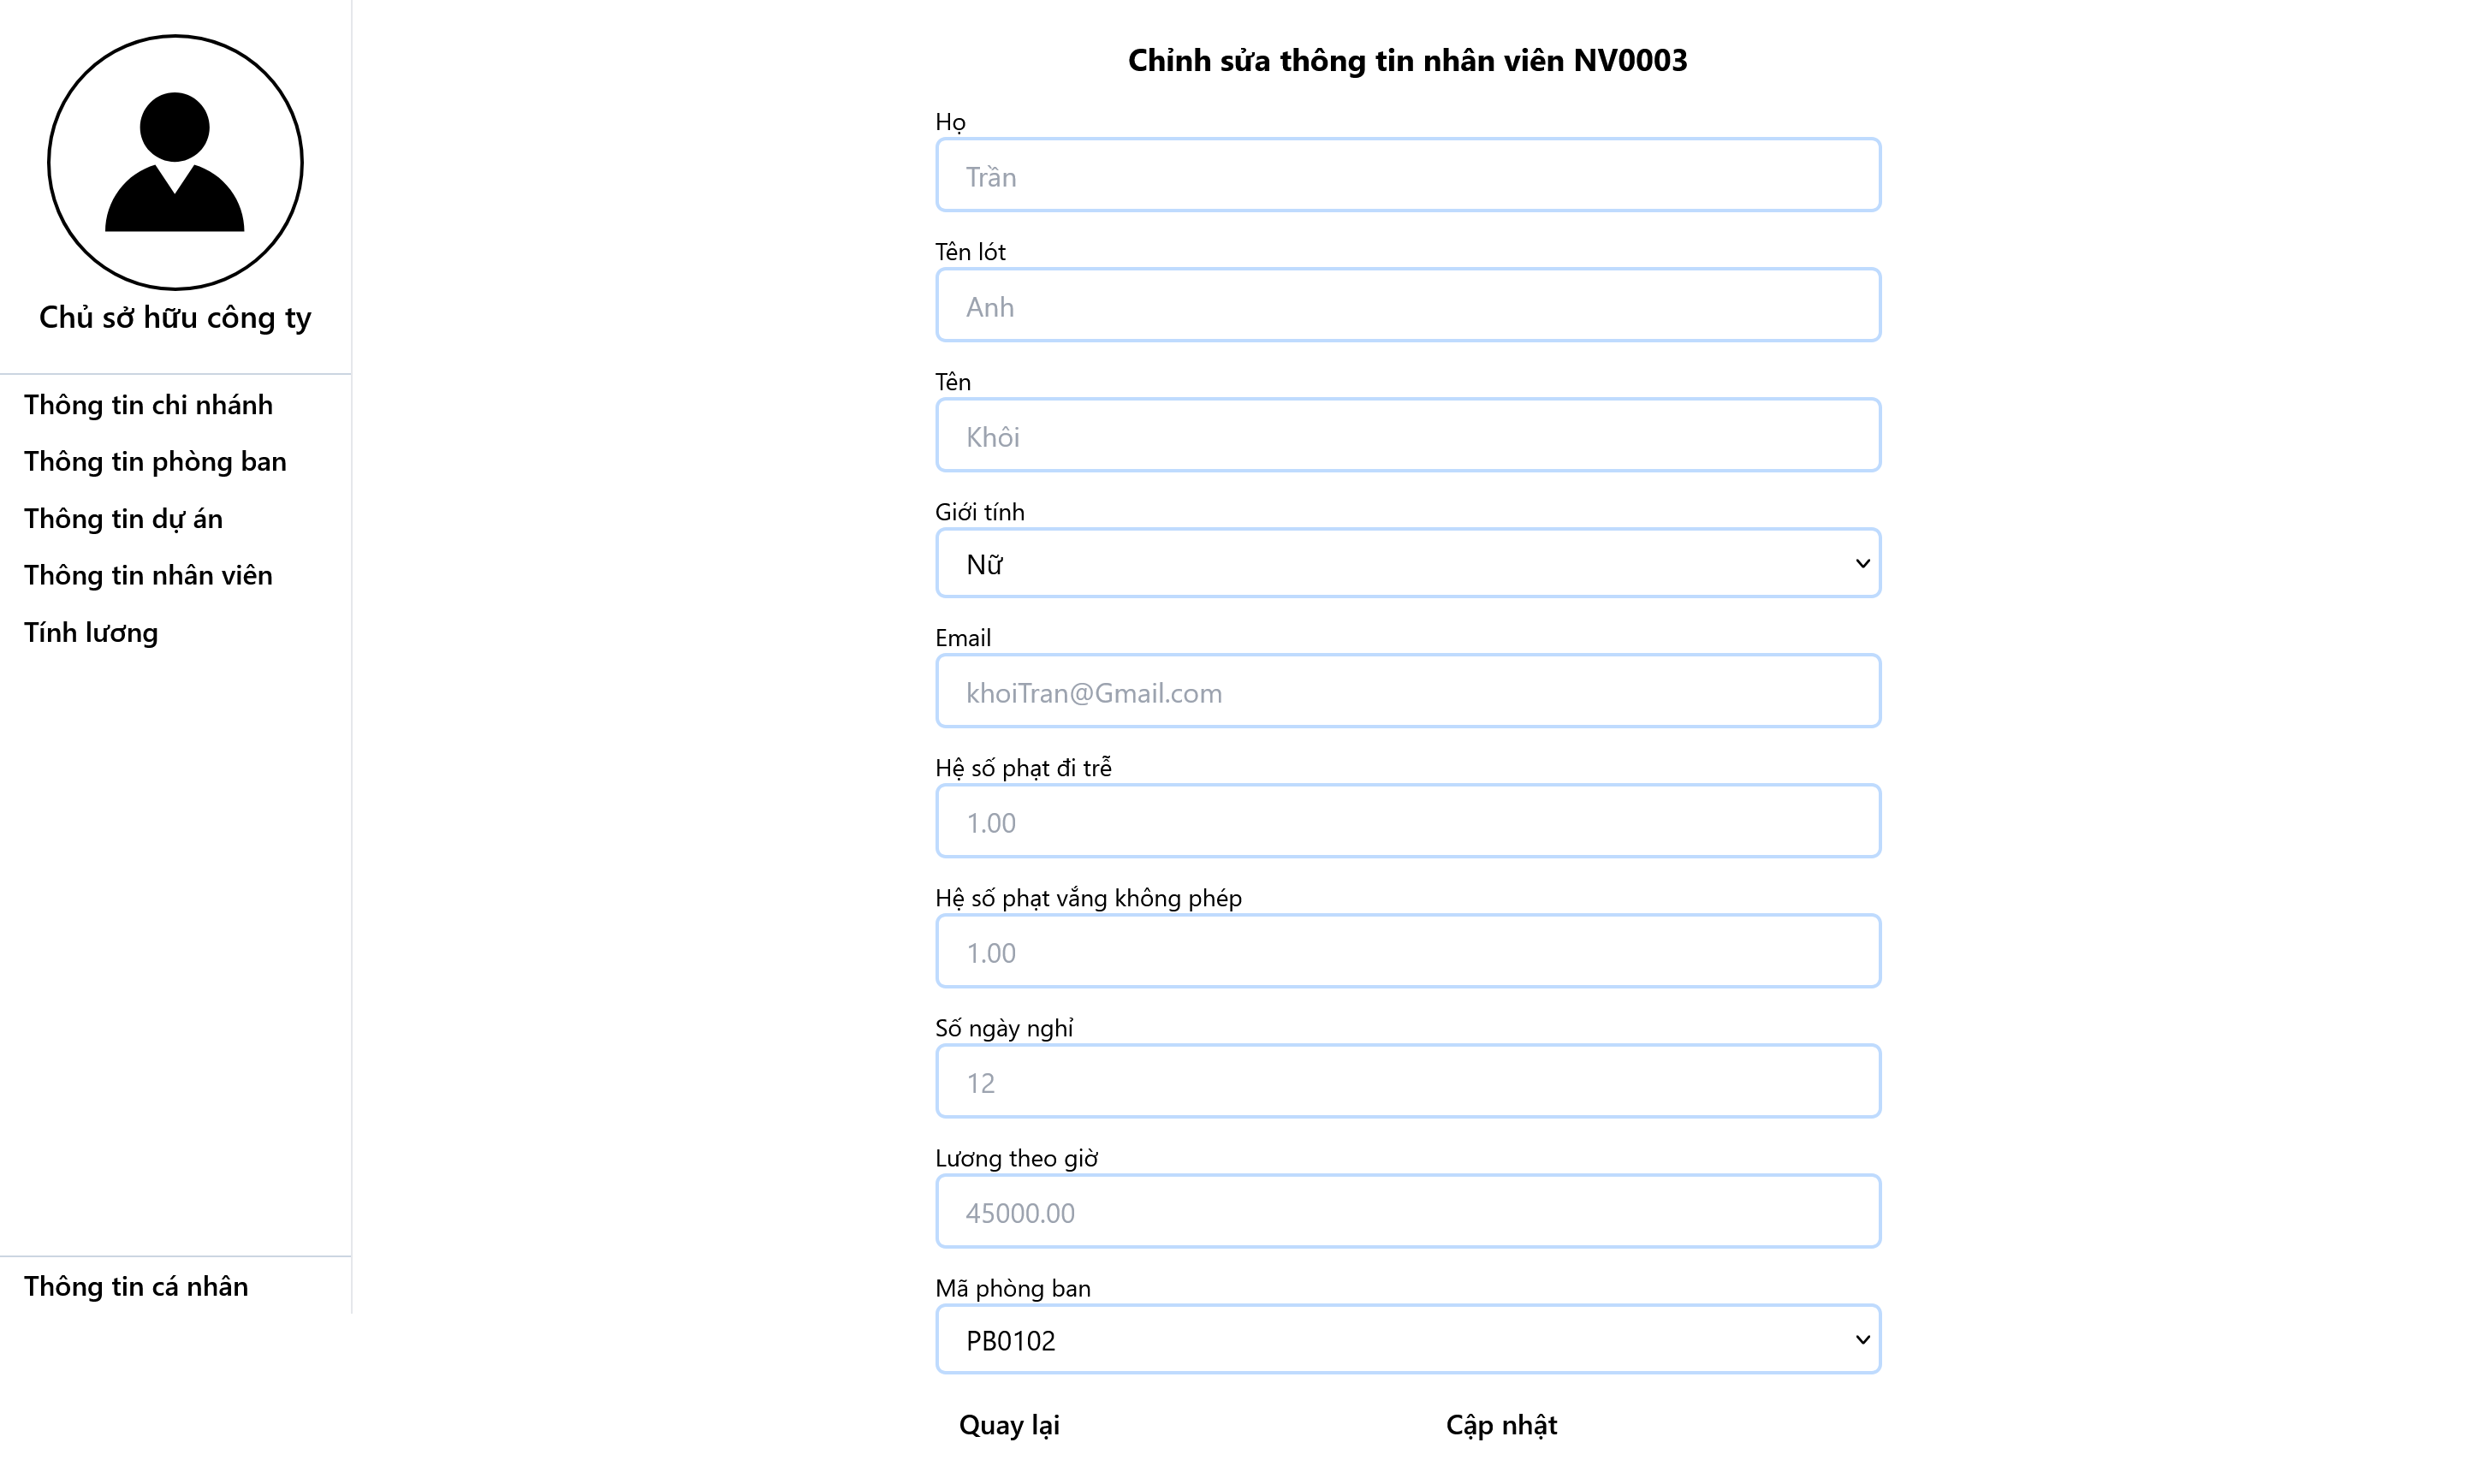
\includegraphics[width=0.75\linewidth]{content/images/ManHinh_1_e.png}
    \caption{Màn hình cập nhật thông tin nhân viên}
    \label{fig:ManHinh_1_e}
\end{figure}

Trường hợp cập nhật nhưng lỗi định dạng ở thuộc tính HeSoPhatDiTre.
\begin{figure}[H]
    \centering
    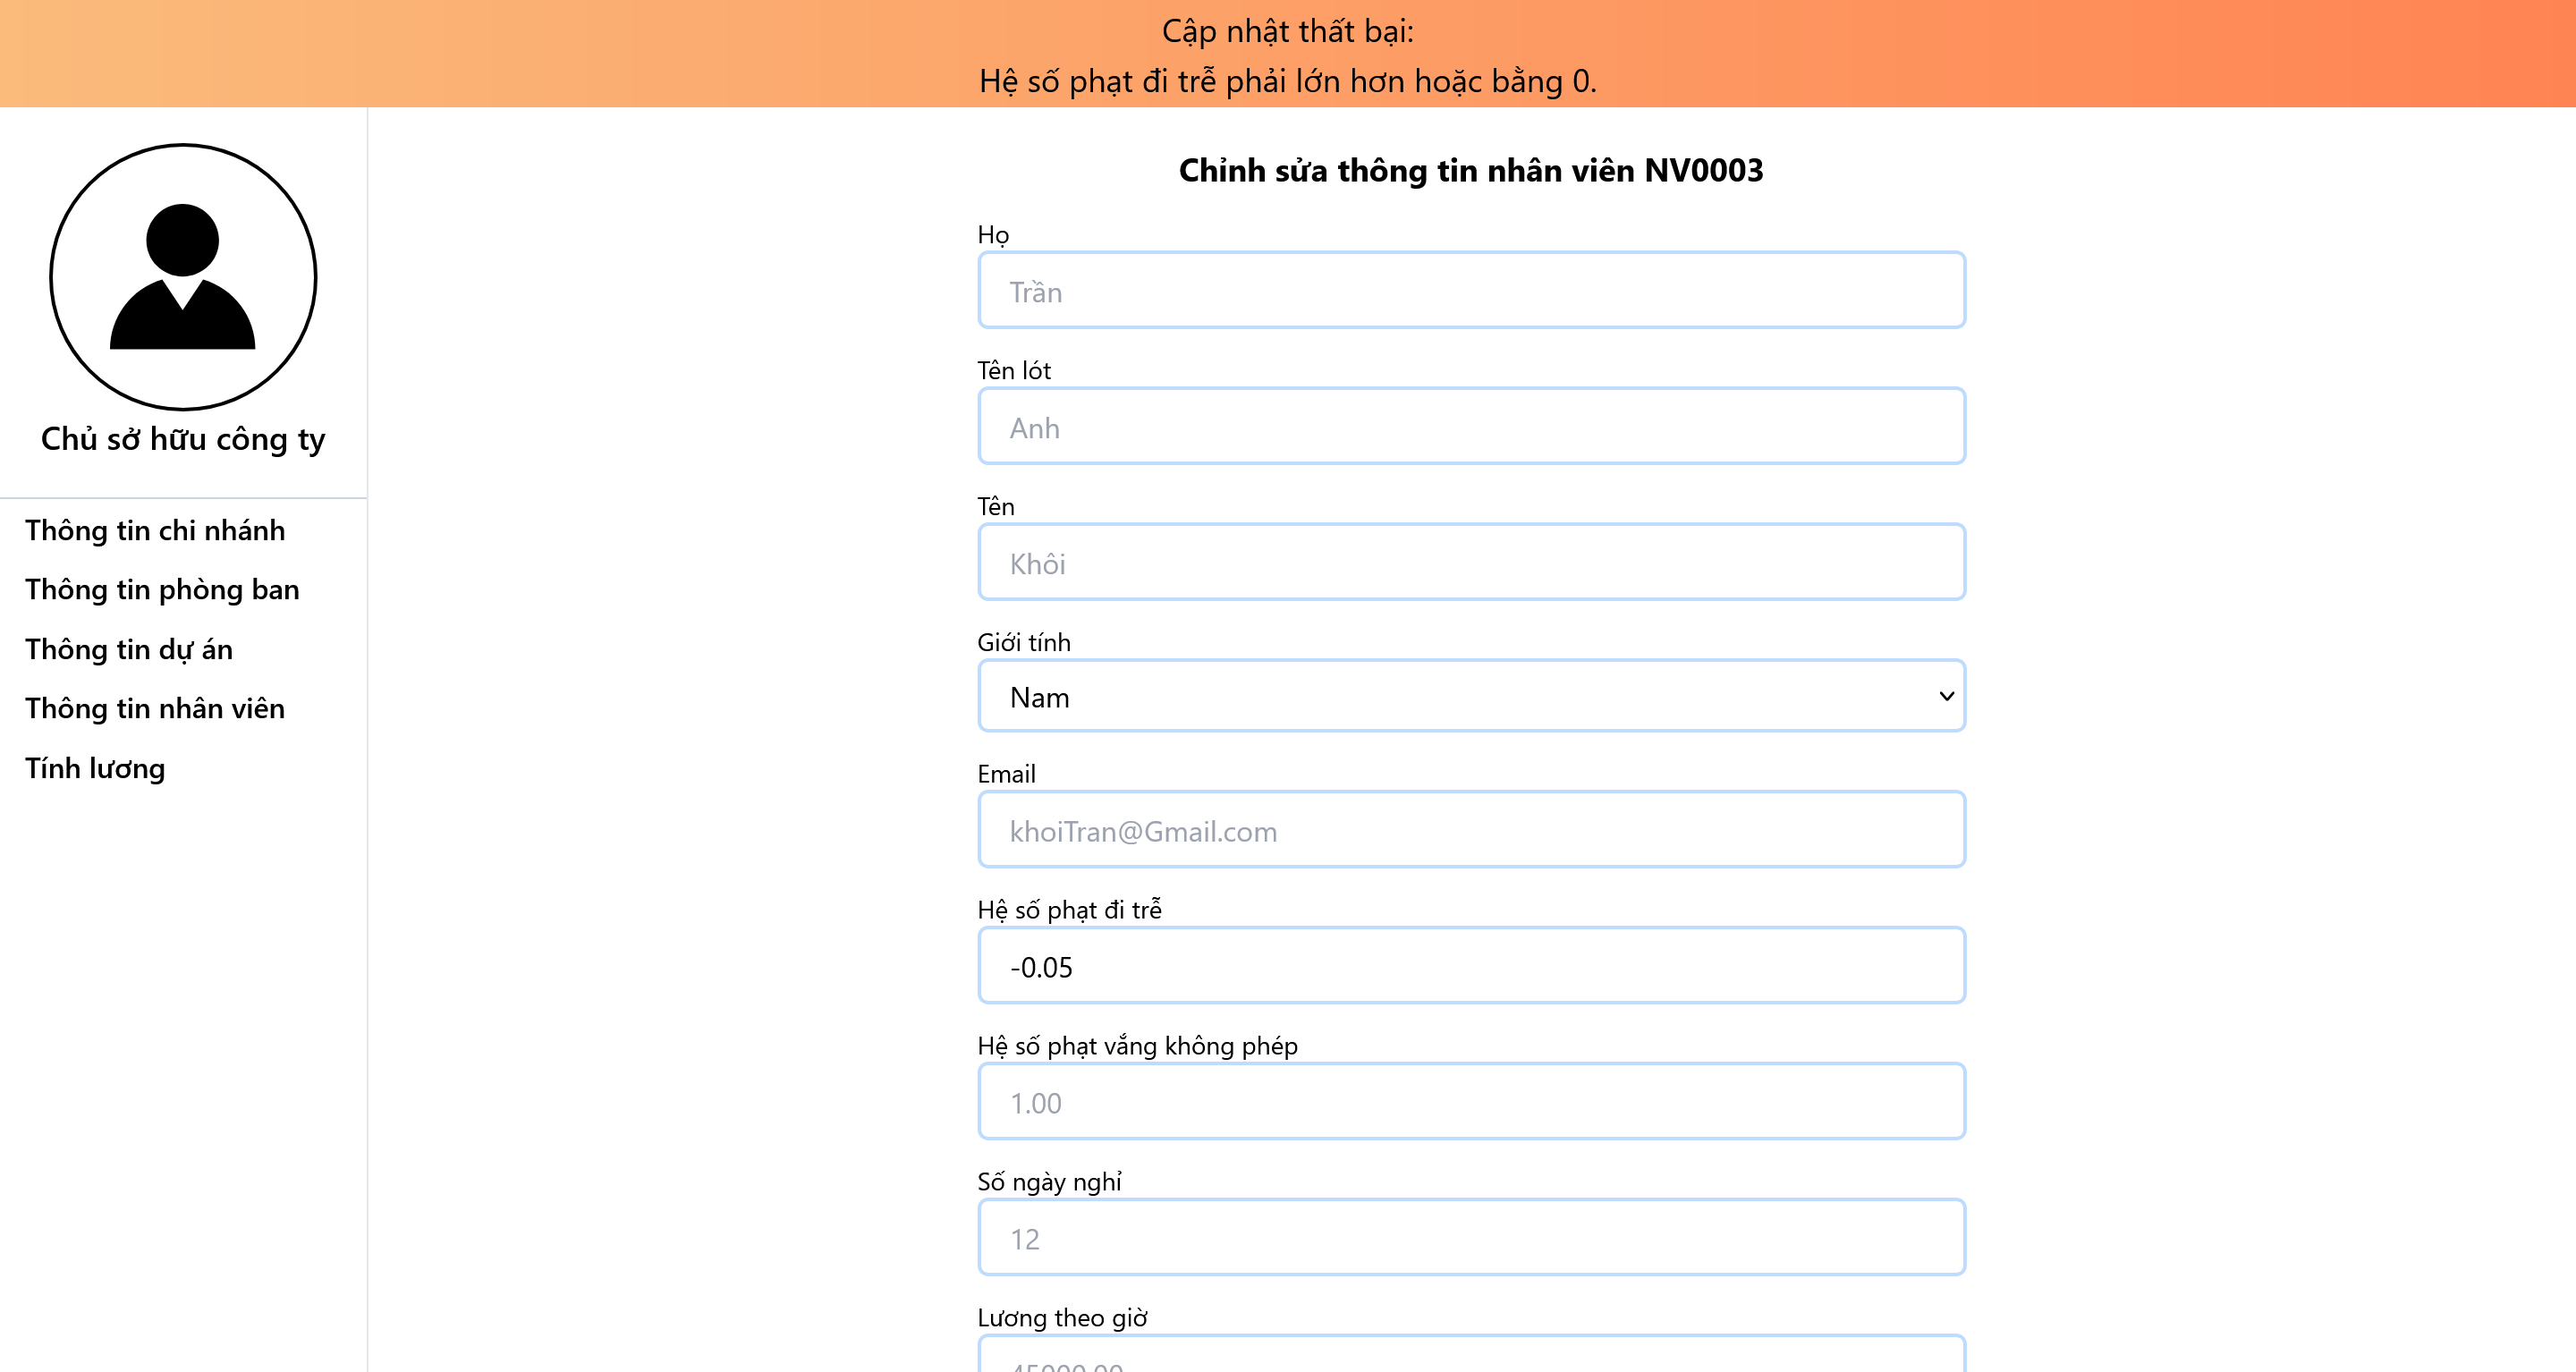
\includegraphics[width=0.75\linewidth]{content/images/ManHinh_1_f.png}
    \caption{Màn hình thông báo lỗi lúc cập nhật thông tin nhân viên}
    \label{fig:ManHinh_1_f}
\end{figure}

Cập nhật thông tin của nhân viên có mã nhân viên là 'NV0003' với các thông tin mới.
\begin{figure}[H]
    \centering
    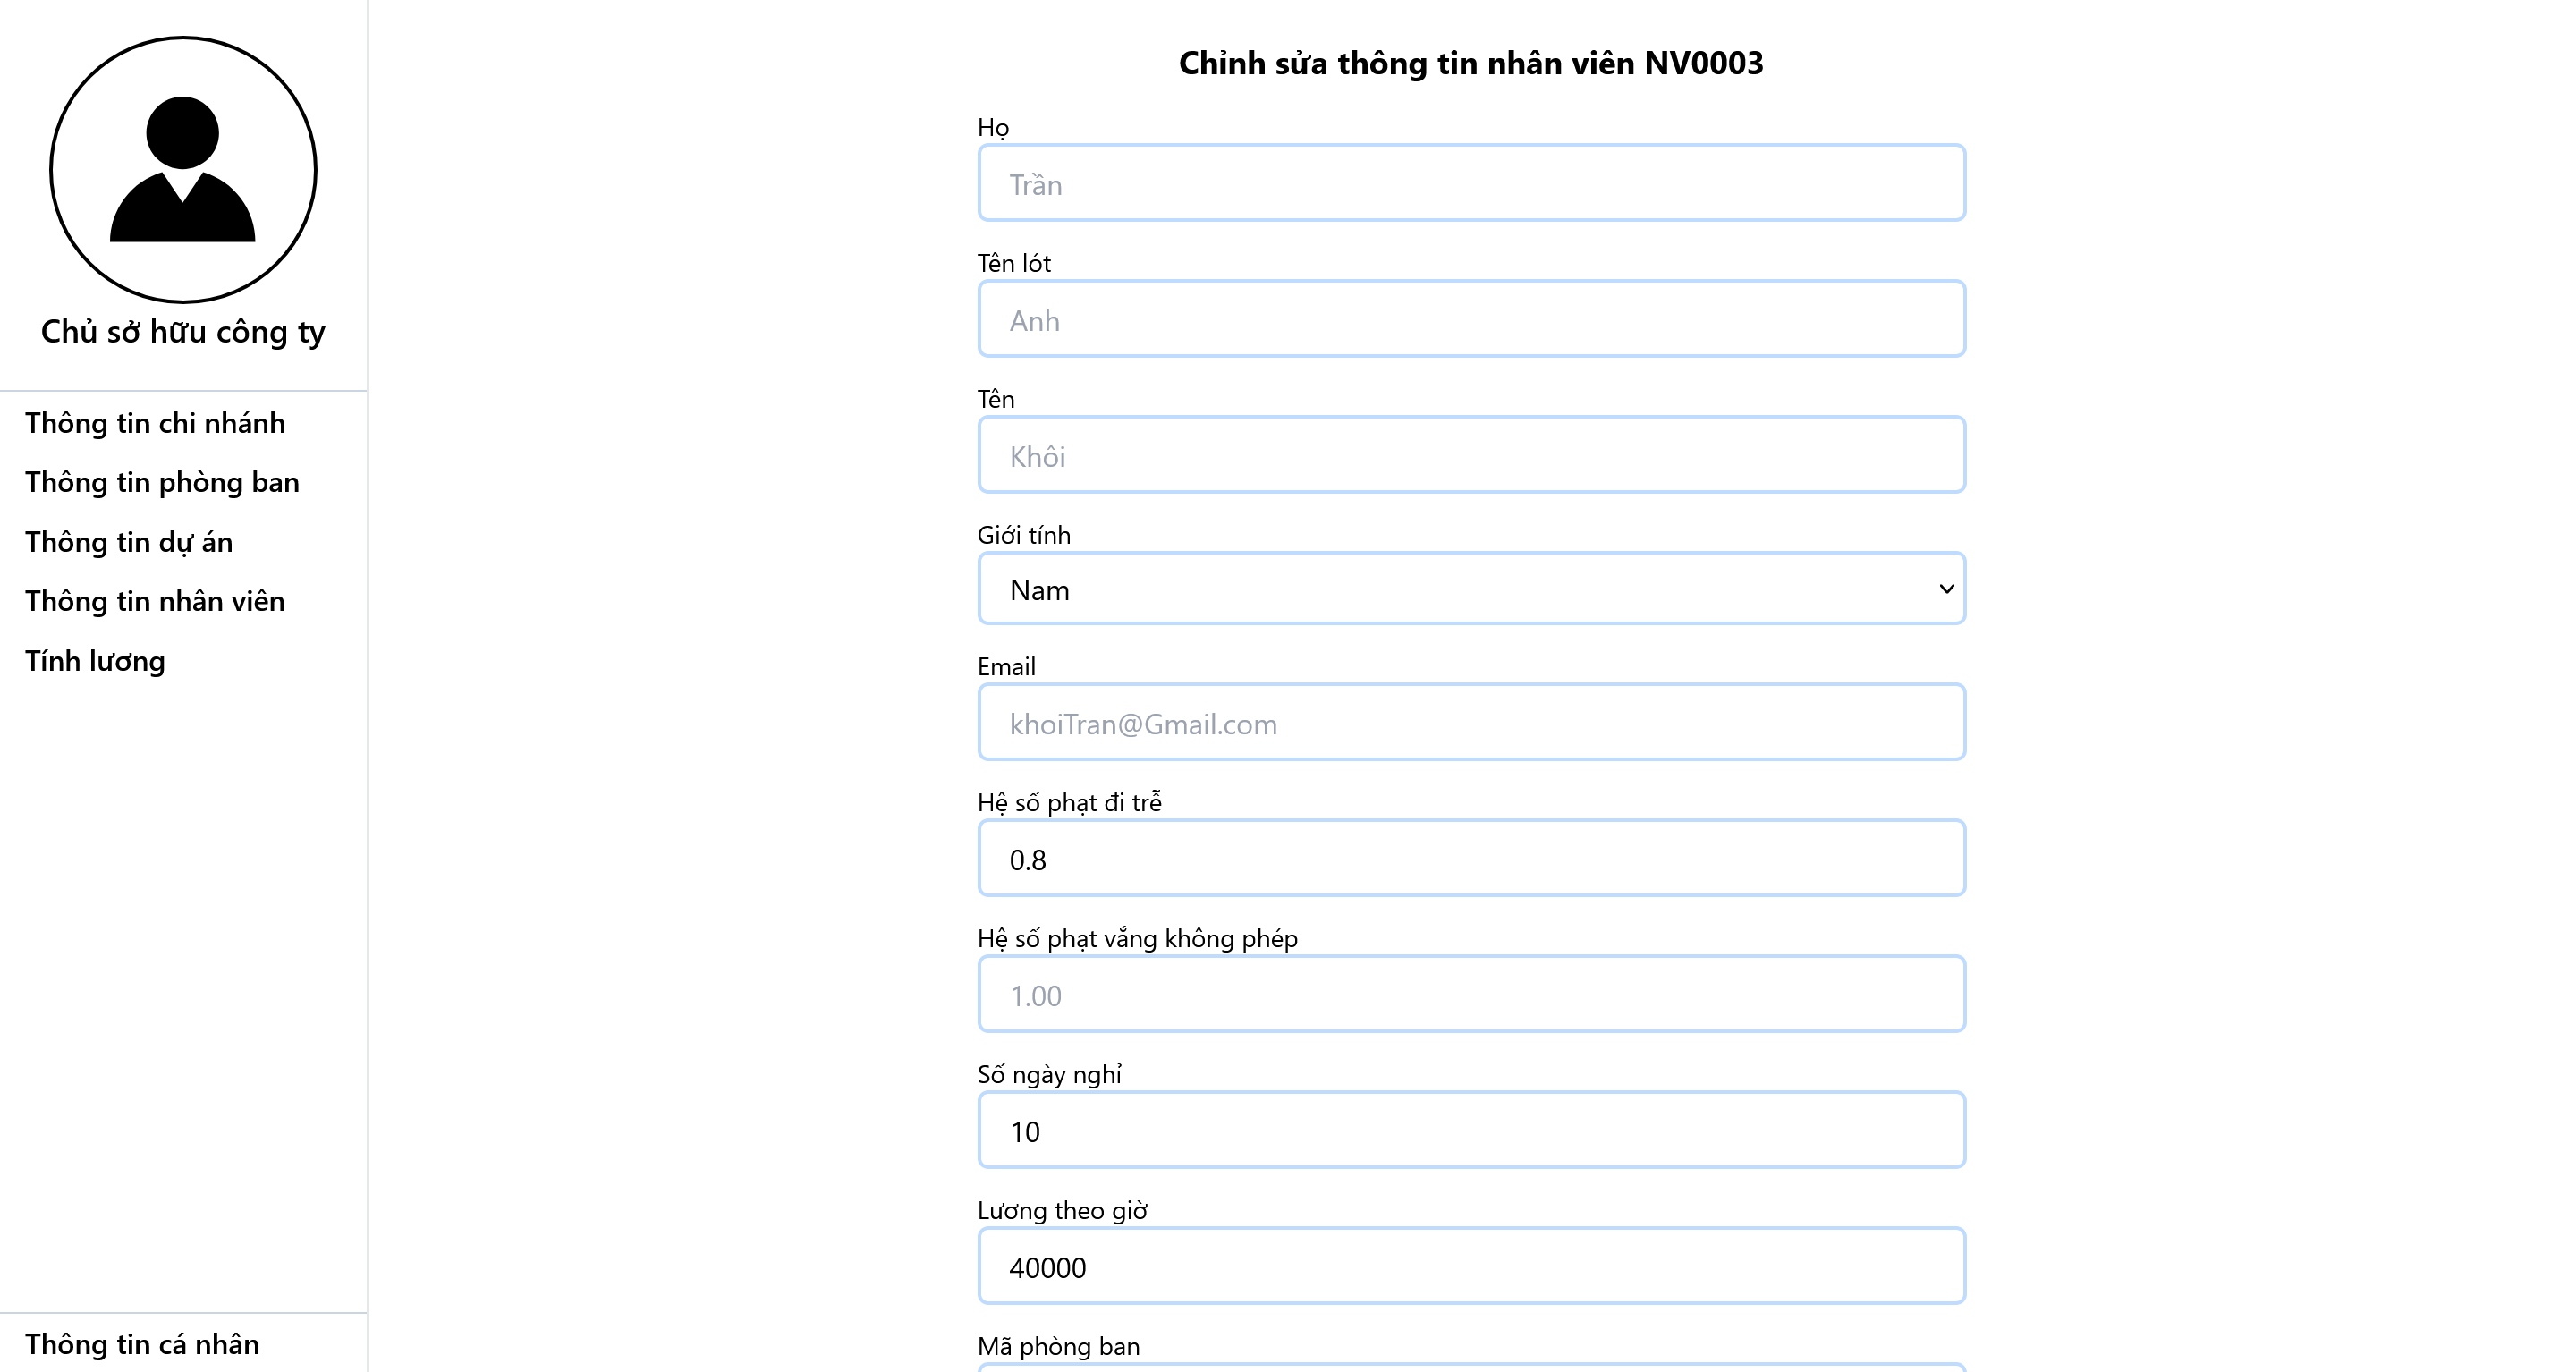
\includegraphics[width=0.75\linewidth]{content/images/ManHinh_1_g.png}
    \caption{Màn hình trước khi nhấn vào nút 'Cập nhật'}
    \label{fig:ManHinh_1_g}
\end{figure}

Kết quả của việc cập nhật thông tin của nhân viên 'NV0003'
\begin{figure}[H]
    \centering
    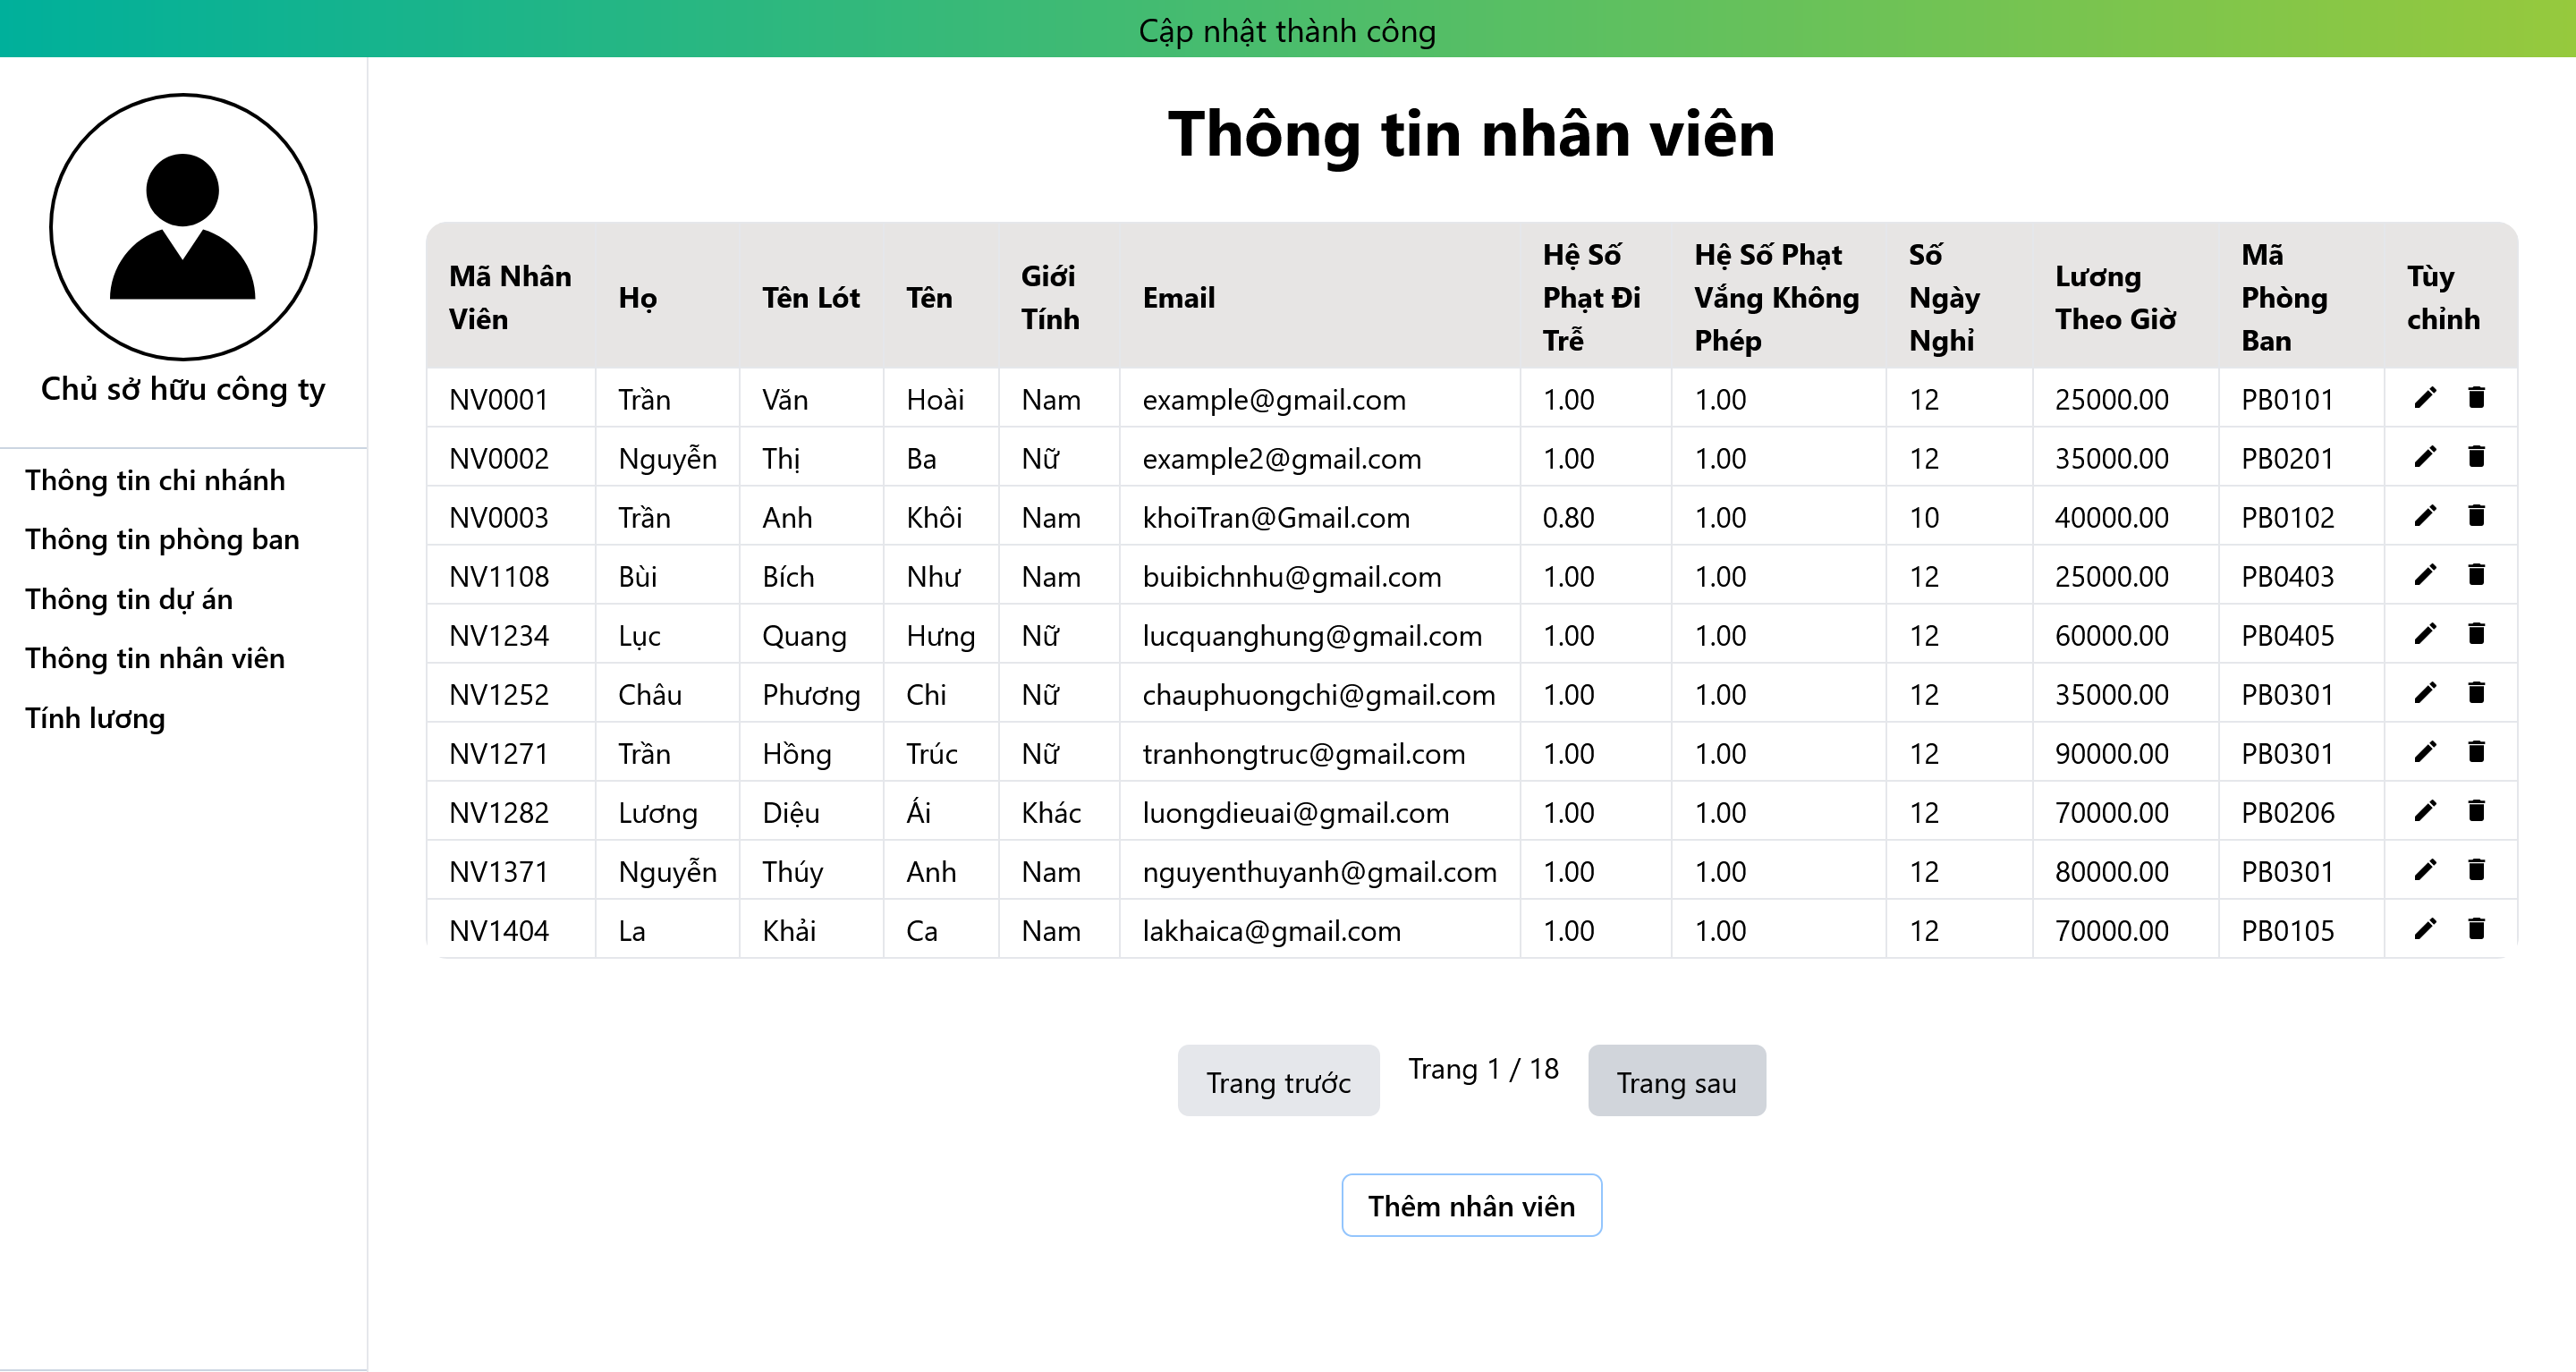
\includegraphics[width=0.75\linewidth]{content/images/ManHinh_1_h.png}
    \caption{Màn hình thông báo cập nhật thông tin nhân viên 'NV0003' thành công}
    \label{fig:ManHinh_1_h}
\end{figure}

Kiểm tra thông tin nhân viên trực tiếp trên cơ sở dữ liệu
\begin{figure}[H]
    \centering
    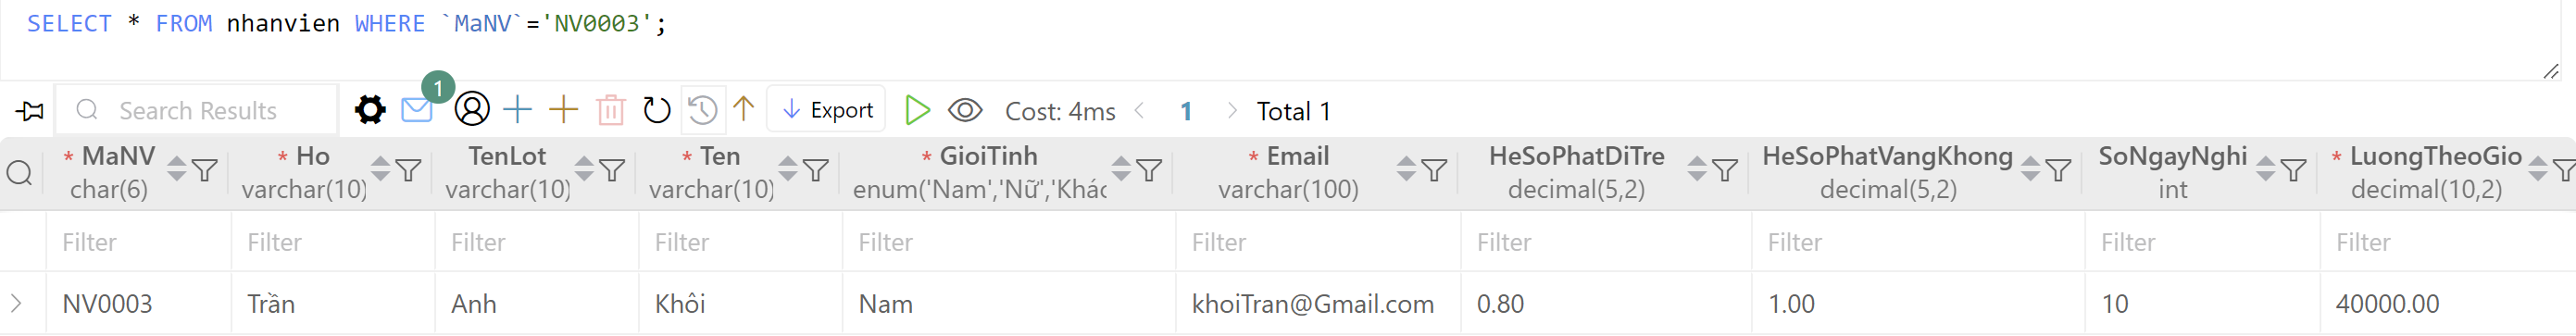
\includegraphics[width=0.75\linewidth]{content/images/ManHinh_1_i.png}
    \caption{Thông tin của nhân viên 'NV0003' đã được cập nhật thành công, với GioiTinh được đổi thành 'Nam', HeSoPhatDiTre được đổi thành 0.08 và LuongTheoGio được đổi thành 40000}
    \label{fig:ManHinh_1_i}
\end{figure}

Để xóa một nhân viên xác định, người dùng tìm đến hàng chứa thông tin nhân viên đó và click vào icon thùng rác. Trang web sẽ hiện ra một bảng cho người dùng xác nhận hành động của mình.
\begin{figure}[H]
    \centering
    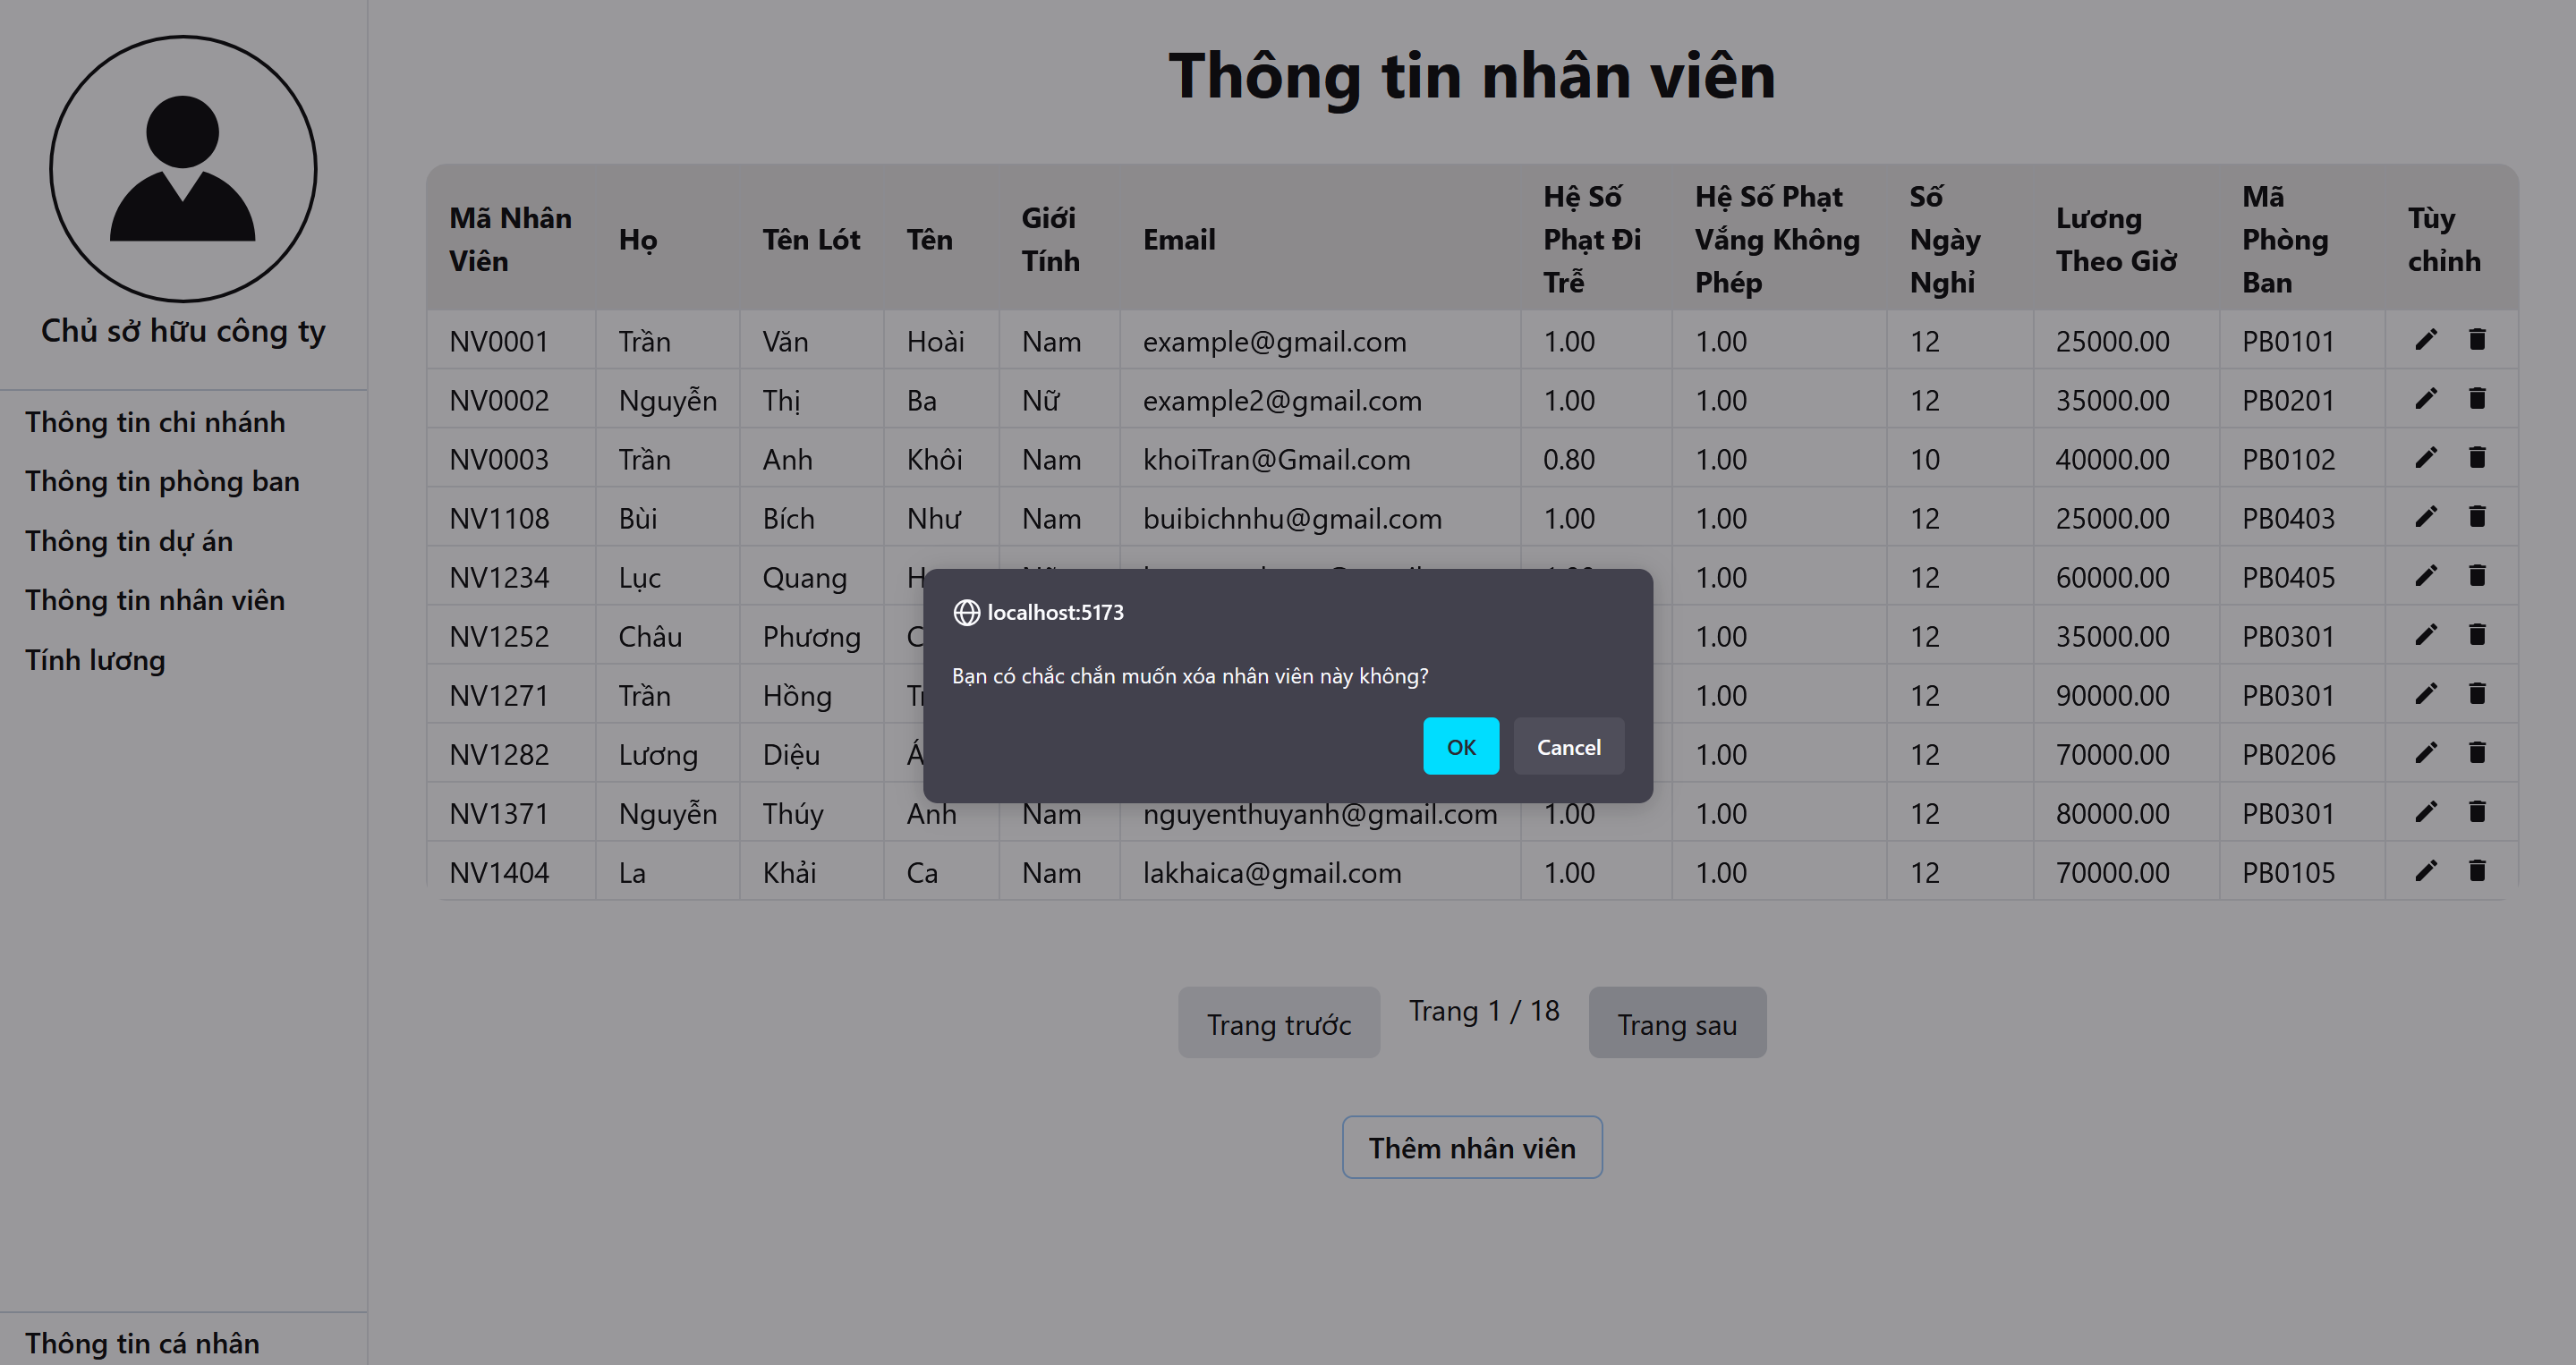
\includegraphics[width=0.75\linewidth]{content/images/ManHinh_1_j.png}
    \caption{Khi click vào icon thùng rác trong hàng chứa mã nhân viên 'NV0003', màn hình hiện lên bảng xác nhận}
    \label{fig:ManHinh_1_j}
\end{figure}

Sau khi xóa nhân viên thành công, màn hình sẽ hiện thị thông báo
\begin{figure}[H]
    \centering
    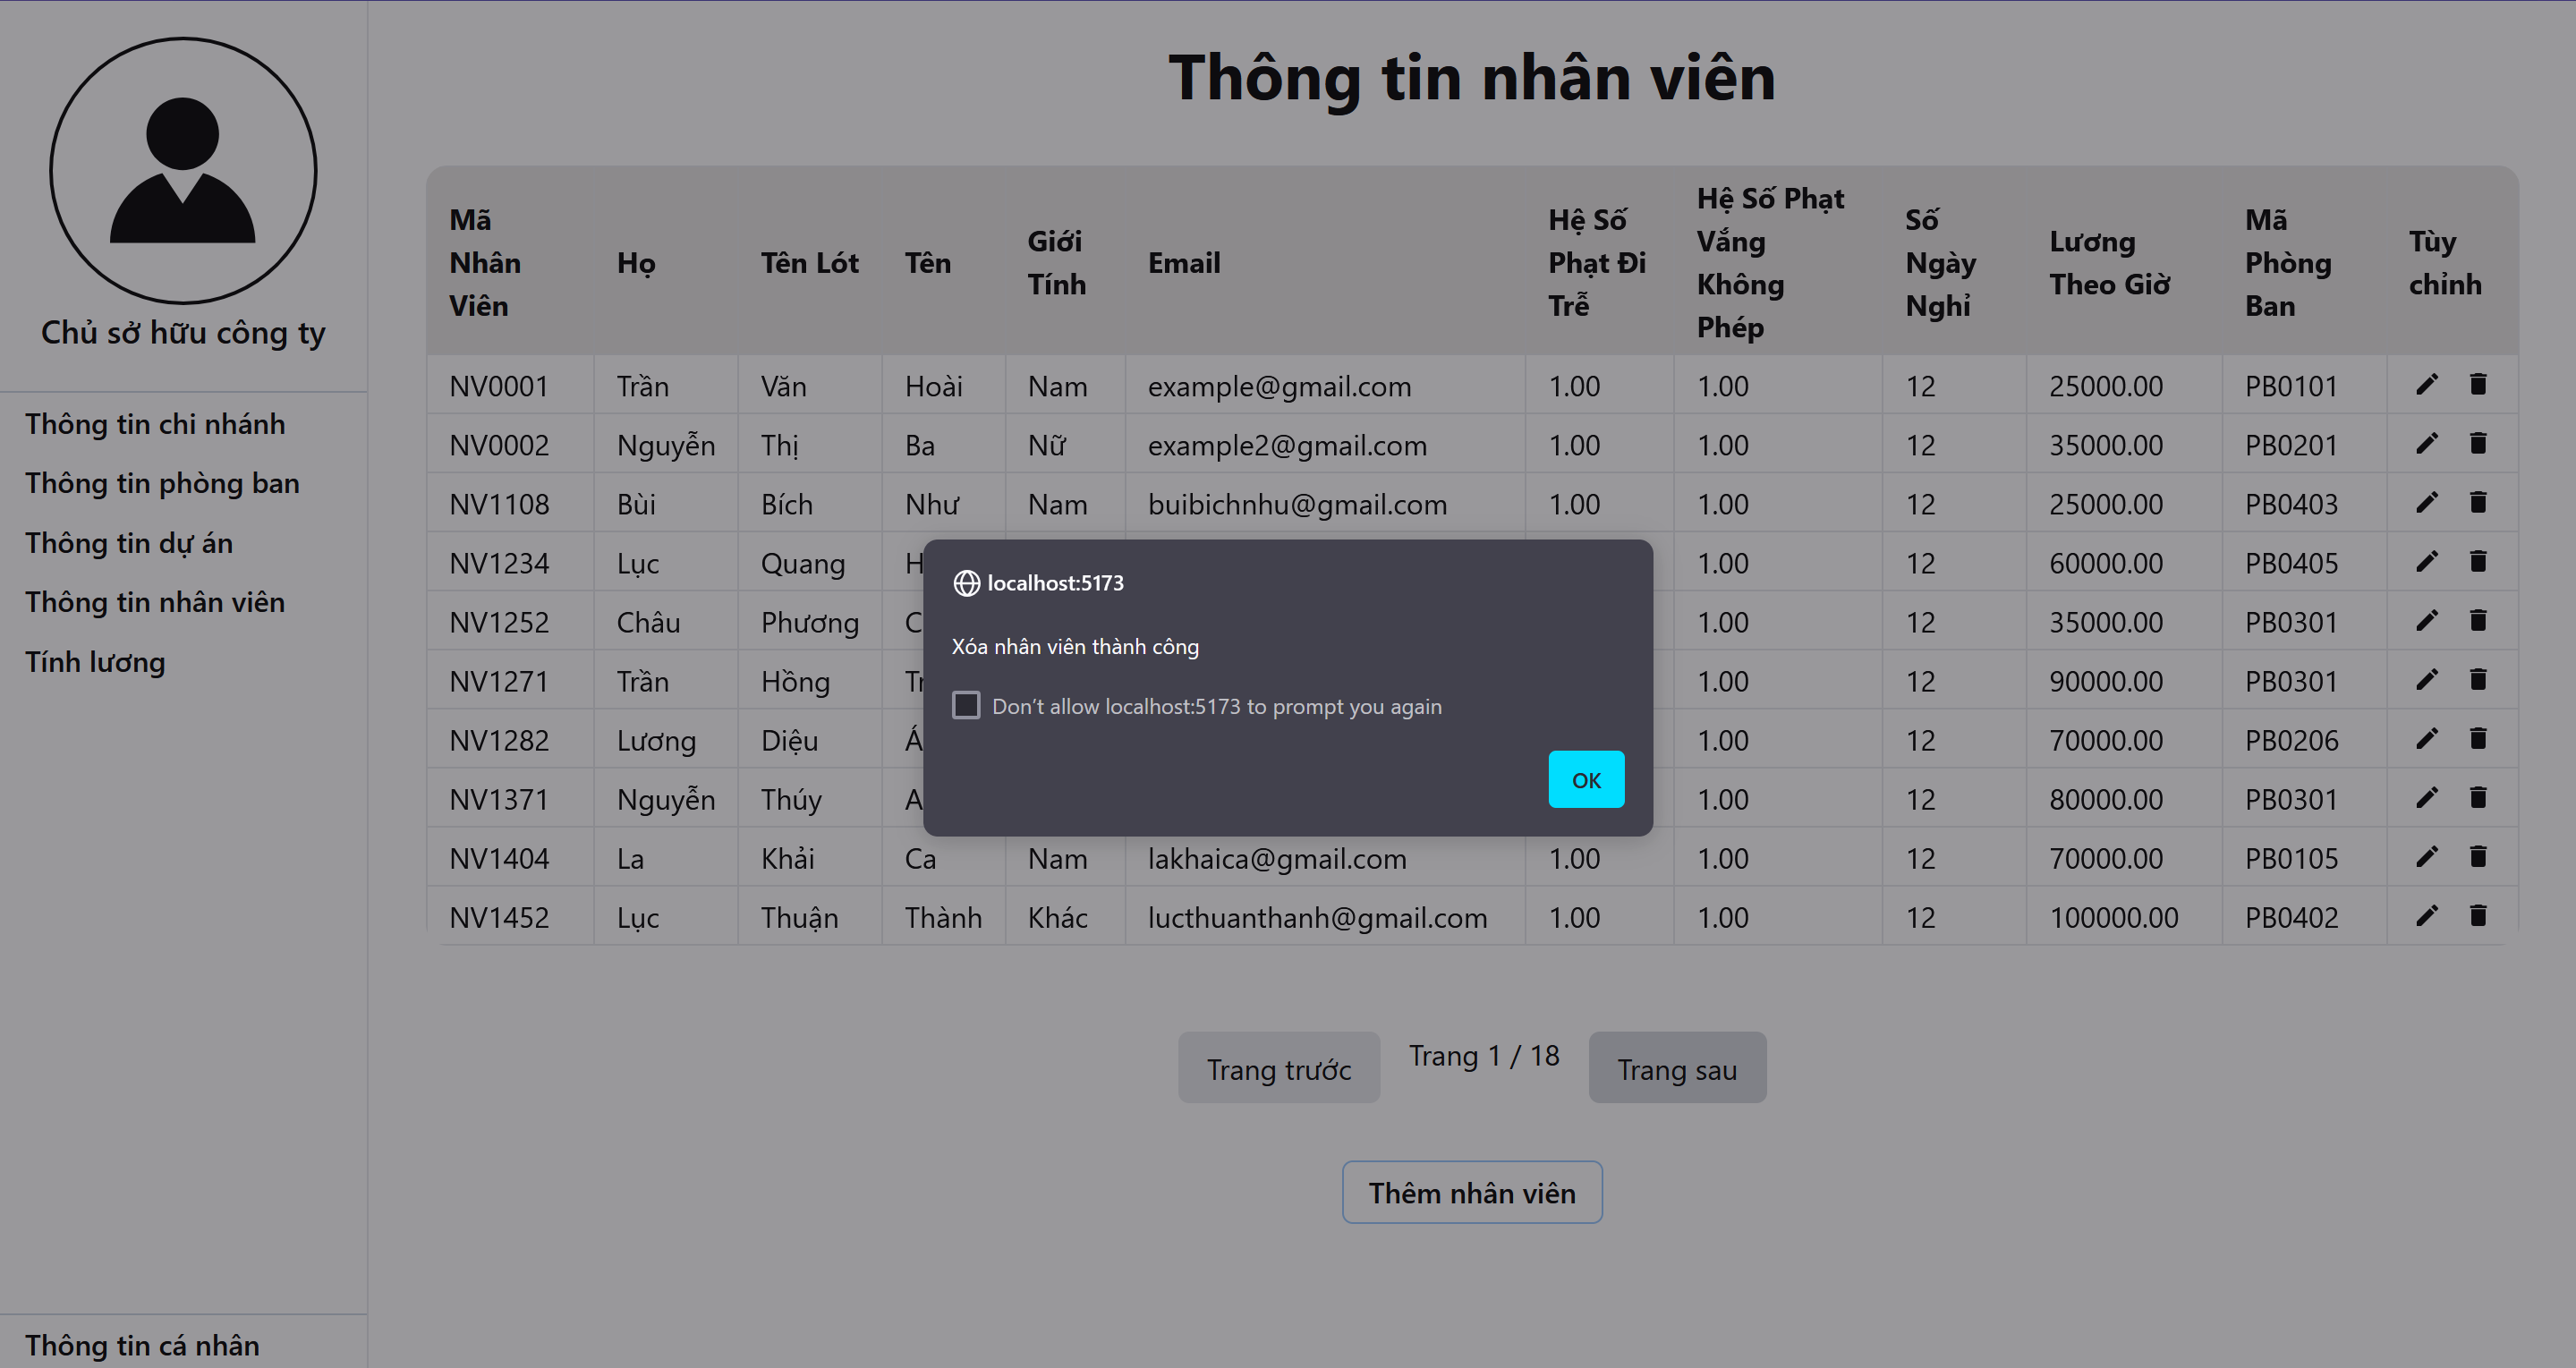
\includegraphics[width=0.75\linewidth]{content/images/ManHinh_1_k.png}
    \caption{Màn hình sau khi xóa nhân viên có mã 'NV0003'}
    \label{fig:ManHinh_1_k}
\end{figure}

Kiểm tra thông tin nhân viên đã bị xóa
\begin{figure}[H]
    \centering
    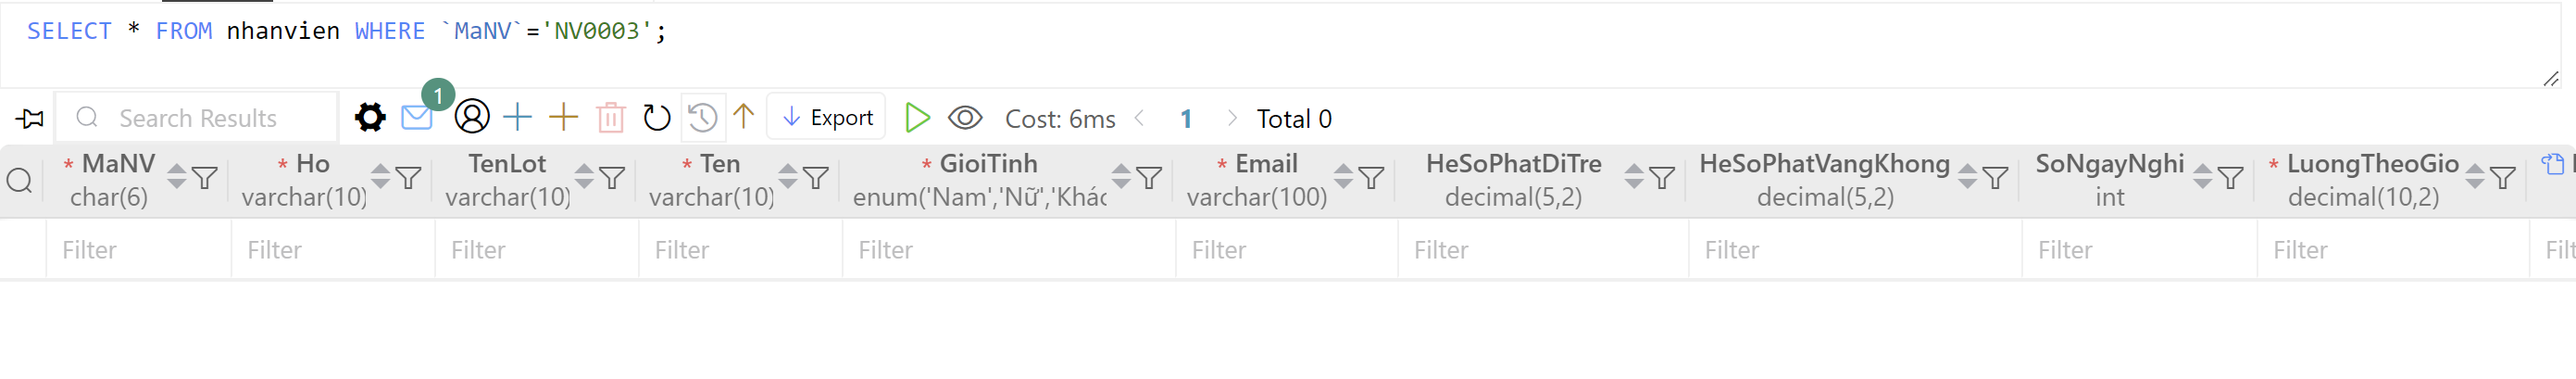
\includegraphics[width=0.75\linewidth]{content/images/ManHinh_1_l.png}
    \caption{Kết quả tra cứu rỗng, chứng tỏ nhân viên 'NV0003' đã bị xóa}
    \label{fig:ManHinh_1_l}
\end{figure}

\newpage
Đoạn code minh họa việc gọi API và render dữ liệu cho màn hình hiển thị bảng thông tin nhân viên
\begin{minted}{javascript}
    // BACKEND
    // API để truy vấn dữ liệu trong bảng nhân viên
    export const getNhanVien = async () => {
        const rows = await ReadQuery('SELECT * FROM NhanVien');
        return rows;
    };

    app.get('/api/nhanvien', async function (req, res) {
        const nhanvien = await getNhanVien();
        res.send({nhanvien})
    })
\end{minted}
\begin{minted}{jsx}
    // FRONTEND
    // lấy dữ liệu từ bảng nhân viên
    try {
      const res = await fetch('/api/nhanvien');
      const data = await res.json();
      // dữ liệu từ bảng nhân viên được lưu trong object NhanVien dưới dạng list
      setNhanVien(data.nhanvien); 
    } catch (error) {
      console.error(error);
    }
    ...
    // truyền dữ liệu xuống component NhanVienTable
    <NhanVienTable rowsData={currentRows} setRowsData={setNhanVien} currentPage={currentPage} />
    ...
    // tại component gốc TableRows, dữ liệu được chuyển thành các một list các <td> và được styling bằng tailwind css
    let row = rowData.map((data, index) => <td className='max-w-[400px] text-wrap px-3 py-1 border' key={index}>{data}</td>);
    // sau đó, chúng được bọc trong element <tr>
    tableRows.push(<tr key={index}>{row}</tr>)
    // cuối cùng, chúng sẽ được render trong tag <tbody> ở cuối file component TableRows.jsx
    return (
        <tbody>
            {tableRows}
        </tbody>
    )
\end{minted}

\newpage
Đoạn code minh họa việc gọi API và render màn hình thêm nhân viên
\begin{minted}{javascript}
    // BACKEND
    // API thêm nhân viên mới
    export const insertNhanVien = async (MaNV, Ho, TenLot, Ten, GioiTinh, Email, LuongTheoGio, MaPhongBan) => {
        const [result, message] = await WriteQuery(
            `CALL ThemNhanVien('${MaNV}', '${Ho}', '${TenLot}', '${Ten}', '${GioiTinh}', '${Email}', ${LuongTheoGio}, '${MaPhongBan}')`
        );
        console.log("result", result)
        return [result, message];
    };

    app.post('/api/nhanvien/insert', async function (req, res) {
        const { MaNV, Ho, TenLot, Ten, GioiTinh, Email, LuongTheoGio, MaPhongBan } = req.body;
        const [result, message] = await insertNhanVien(MaNV, Ho, TenLot, Ten, GioiTinh, Email, LuongTheoGio, MaPhongBan);
        if (result === 400) {
            return res.status(400).json({
                success: false,
                message: message
            });
        }
        return res.status(200).json({
            success: true,
            message: 'Thêm nhân viên thành công'
        });
    });
\end{minted}
\begin{minted}{jsx}
    // FRONTEND
    // Khởi tạo thực thể newNhanVien, chứa các thông tin nhân viên mới sẽ được thêm vào công ty
    const [newNhanVien, setNewNhanVien] = useState({
        MaNV: '',
        Ho: '',
        TenLot: '',
        Ten: '',
        GioiTinh: '',
        Email: '',
        LuongTheoGio: '',
        MaPhongBan: ''
    });

    // các input fields và nút 'Thêm nhân viên'
    // Khi người dùng thay đổi giá trị ở các input fields, giá trị của các trường trong thực thể newNhanVien sẽ được thay đổi dựa trên các hàm trong onChangeHandle
    <InputField label={'Mã nhân viên'} placeholder={'NVxxxx'} type={'text'} onChangeHandle={handleSetMaNV} />
    <InputField label={'Họ'} placeholder={'Nguyễn'} type={'text'} onChangeHandle={handleSetHo} />
    <InputField label={'Tên lót'} placeholder={'Văn'} type={'text'} onChangeHandle={handleSetTenLot} />
    <InputField label={'Tên'} placeholder={'A'} type={'text'} onChangeHandle={handleSetTen} />
    <SelectField label={'Giới tính'} options={['Nam', 'Nữ', 'Khác']} onchangeHandler={handleSetGioiTinh} />
    <InputField label={'Email'} placeholder={'example@domain.com'} type={'email'} onChangeHandle={handleSetEmail} />
    <InputField label={'Lương theo giờ'} placeholder={'20000'} type={'number'} onChangeHandle={handleSetLuongTheoGio} />
    <SelectField label={'Mã phòng ban'} options={phongBanOptions} onchangeHandler={handleSetMaPhongBan} />
    
    <div className='my-3 w-fit border-blue-300 border rounded-md'>
        <Button label={'Thêm nhân viên'} onClickFunction={handleAddNhanVien} />
    </div>
\end{minted}
\begin{minted}{jsx}
    // Hàm thực thi lệnh thêm nhân viên
    const createNhanVien = async (nhanVien) => {
        const errors = [];
    
        // Kiểm tra thiếu trường bắt buộc (trừ trường Tên lót)
        if (!nhanVien.MaNV || !nhanVien.Ho || !nhanVien.Ten || !nhanVien.GioiTinh || !nhanVien.Email || !nhanVien.LuongTheoGio || !nhanVien.MaPhongBan) {
        errors.push('Hãy điền vào tất cả các trường.');
        }
    
        // Kiểm tra định dạng cụ thể
        if (nhanVien.MaNV && !nhanVien.MaNV.match(/^NV[0-9]{4}$/)) {
        errors.push('Mã nhân viên phải có định dạng NVxxxx, với 4 chữ số.');
        }
    
        if (nhanVien.Email && !nhanVien.Email.match(/^[a-zA-Z0-9._%+-]+@[a-zA-Z0-9.-]+\.[a-zA-Z]{2,}$/)) {
        errors.push('Email không đúng định dạng.');
        }
    
        if (nhanVien.Ho && nhanVien.Ho.match(/[^a-zA-ZÀ-ỹ ]/)) {
        errors.push('Họ không được chứa số hoặc ký tự đặc biệt.');
        }
    
        if (nhanVien.Ten && nhanVien.Ten.match(/[^a-zA-ZÀ-ỹ ]/)) {
        errors.push('Tên không được chứa số hoặc ký tự đặc biệt.');
        }
    
        if (nhanVien.LuongTheoGio && parseFloat(nhanVien.LuongTheoGio) <= 0) {
        errors.push('Lương theo giờ phải lớn hơn 0.');
        }
    
        // Nếu có lỗi, trả về danh sách lỗi
        if (errors.length > 0) {
        return {
            success: false,
            message: errors.join('\n') // Kết hợp các lỗi thành một chuỗi
        };
        }
    
        // Nếu không có lỗi, gửi yêu cầu tới API để thêm nhân viên
        const res = await fetch('/api/nhanvien/insert', {
            method: 'POST',
            headers: {'Content-Type': 'application/json'},
            body: JSON.stringify(nhanVien)
        });
\end{minted}
\begin{minted}[firstnumber=45]{jsx}
        const data = await res.json();
        return {
        success: data.success,
        message: data.message
        };
    };
\end{minted}

\newpage
Đoạn code minh họa cho việc gọi API và render màn hình chỉnh sửa nhân viên
\begin{minted}{javascript}
    // BACKEND
    // API để lấy thông tin của một nhân viên theo mã nhân viên
    export const getNhanVienByMaNV = async (MaNV) => {
        const rows = await ReadQuery(`SELECT * FROM NhanVien WHERE MaNV = '${MaNV}'`);
        return rows.length ? rows[0] : null;
    };

    app.get('/api/nhanvien/:MaNV', async (req, res) => {
        const { MaNV } = req.params;
        try {
        const nhanvien = await getNhanVienByMaNV(MaNV); // Hàm này cần lấy từ database
        if (!nhanvien) {
            return res.status(404).json({ success: false, message: 'Nhân viên không tồn tại' });
        }
        res.status(200).json({ success: true, nhanvien });
        } catch (error) {
        console.error(error);
        res.status(500).json({ success: false, message: 'Lỗi server' });
        }
    });

    // API để cập nhật thông tin một nhân viên
    export const updateNhanVien = async (MaNV, Ho, TenLot, Ten, GioiTinh, Email, HeSoPhatDiTre, HeSoPhatVangKhongPhep, SoNgayNghi, LuongTheoGio, MaPhongBan) => {
        const [result, message] = await WriteQuery(
            `CALL SuaNhanVien('${MaNV}', '${Ho}', '${TenLot}', '${Ten}', '${GioiTinh}', '${Email}', ${HeSoPhatDiTre}, ${HeSoPhatVangKhongPhep}, ${SoNgayNghi}, ${LuongTheoGio}, '${MaPhongBan}')`
        );
        console.log("result", result)
        return [result, message];
    };
\end{minted}
\begin{minted}[firstnumber=30]{javascript}
    app.put('/api/nhanvien/update/:MaNV', async (req, res) => {
        const { MaNV, Ho, TenLot, Ten, GioiTinh, Email, HeSoPhatDiTre, HeSoPhatVangKhongPhep, SoNgayNghi, LuongTheoGio, MaPhongBan } = req.body;
        console.log("Dữ liệu nhận được từ frontend:", req.body); // Kiểm tra dữ liệu từ frontend
        try {
            const [result, message] = await updateNhanVien(MaNV, Ho, TenLot, Ten, GioiTinh, Email, HeSoPhatDiTre, HeSoPhatVangKhongPhep, SoNgayNghi, LuongTheoGio, MaPhongBan);
            console.log("Kết quả cập nhật:", result); // Log kết quả từ database
            if (result === 400) {
                return res.status(400).json({ success: false, message });
            }
            res.status(200).json({ success: true, message: 'Cập nhật thành công' });
        } catch (error) {
            console.error(error);
            res.status(500).json({ success: false, message: 'Lỗi server' });
        }
    });
\end{minted}
\begin{minted}{jsx}
    // Lấy thông tin của nhân viên để hiển thị thông tin hiện tại dưới dạng placeholder của các input fields
    const fetchNhanVien = async () => {
        try {
            const res = await fetch(`/api/nhanvien/${MaNV}`); // API lấy thông tin nhân viên
            const data = await res.json();
            if (data.success) {
                const nhanVienData = data.nhanvien;
                setNhanVien({
                    Ho: nhanVienData[1],
                    TenLot: nhanVienData[2],
                    Ten: nhanVienData[3],
                    GioiTinh: nhanVienData[4],
                    Email: nhanVienData[5],
                    HeSoPhatDiTre: nhanVienData[6],
                    HeSoPhatVangKhongPhep: nhanVienData[7],
                    SoNgayNghi: nhanVienData[8],
                    LuongTheoGio: nhanVienData[9],
                    MaPhongBan: nhanVienData[10],
                });
            } else {
                console.error(data.message);
                alert('Không tìm thấy nhân viên!');
                navigate('/nhan-vien');
            }
        } catch (error) {
            console.error('Error fetching nhân viên:', error.message);
            alert('Có lỗi xảy ra khi lấy thông tin nhân viên!');
        }
    };
    // Đoạn code hiển thị các input fields

    // Thực thể để lưu thông tin mới của nhân viên
    // Khi các giá trị trong input fields được thay đổi, các trường của thực thể nhanVien cũng thay đổi theo dựa trên hàm setNhanVien().
    const [nhanVien, setNhanVien] = useState({
        Ho: '',
        TenLot: '',
        Ten: '',
        GioiTinh: '',
        Email: '',
        HeSoPhatDiTre: '',
        HeSoPhatVangKhongPhep: '',
        SoNgayNghi: '',
        LuongTheoGio: '',
        MaPhongBan: '',
    });
\end{minted}
\begin{minted}[firstnumber=46]{jsx}
    // Hàm thực hiện việc gọi API cập nhật thông tin
    const handleUpdateNhanVien = async () => {
        // Các lỗi về nhập liệu sẽ được kiểm tra bằng hàm validateNhanVien và được lưu vào thực thể errors
        const errors = validateNhanVien(nhanVien);
        if (errors.length > 0) {
            // Đoạn code thông báo lỗi
            return;
        }

        const updatedNhanVien = {
            MaNV, // Mã nhân viên từ URL (không thay đổi)
            ...nhanVien,
            HeSoPhatDiTre: parseFloat(nhanVien.HeSoPhatDiTre),
            HeSoPhatVangKhongPhep: parseFloat(nhanVien.HeSoPhatVangKhongPhep),
            SoNgayNghi: parseInt(nhanVien.SoNgayNghi, 10),
            LuongTheoGio: parseFloat(nhanVien.LuongTheoGio),
        };

        try {
            const res = await fetch(`/api/nhanvien/update/${MaNV}`, {
                method: 'PUT',
                headers: {
                'Content-Type': 'application/json',
                },
                body: JSON.stringify(updatedNhanVien),
            });
            const data = await res.json();

            if (data.success) {
                // Đoạn code hiển thị thông báo cập nhật thành công
                navigate(`/nhan-vien?page=${currentPage}`); // Quay lại trang đúng
            } else {
                // Đoạn code hiển thị thông báo cập nhật thất bại
            }
        } catch (error) {
            console.error('Error updating nhân viên:', error.message);
        }
    };
\end{minted}

\newpage
Đoạn code minh họa cho việc gọi API cho thao tác xóa một nhân viên
\begin{minted}{javascript}
    // API cho thao tác xóa một nhân viên cụ thể
    export const deleteNhanVien = async (MaNV) => {
        const [result, message] = await WriteQuery(`CALL XoaNhanVien('${MaNV}')`);
        return [result, message];
    };

    app.delete('/api/nhanvien/delete/:MaNV', async function (req, res) {
        const { MaNV } = req.params;
        console.log(`Đang thực hiện yêu cầu xóa nhân viên với MãNV: ${MaNV}`);
        const [result, message] = await deleteNhanVien(MaNV);
        if (result === 400) {
            return res.status(400).json({
                success: false,
                message: message
            });
        }
        return res.status(200).json({
            success: true,
            message: 'Xóa nhân viên thành công'
        });
    });

    // Khi click vào icon thùng rác ở một hàng trong bảng nhân viên, Mã nhân viên của hàng đó sẽ được truyền để làm tham số cho hàm xóa nhân viên dưới đây
    const deleteFunction = async (MaNV) => {
        if (window.confirm('Bạn có chắc chắn muốn xóa nhân viên này không?')) {
            // Xóa tạm thời hàng khỏi giao diện trước
            setRowsData((prevRows) => prevRows.filter((row) => row[0] !== MaNV));
        
            try {
                const res = await fetch(`/api/nhanvien/delete/${MaNV}`, {
                method: 'DELETE',
                });
                const data = await res.json();
\end{minted}
\begin{minted}[firstnumber=34]{javascript}
                if (data.success) {
                    alert('Xóa nhân viên thành công');
                    } else {
                    alert('Xóa nhân viên không thành công: ' + data.message);
                    // Khôi phục lại hàng nếu xóa không thành công
                    setRowsData((prevRows) => [...prevRows, rowsData.find((row) => row[0] === MaNV)]);
                    }
                } catch (error) {
                    console.error('Error deleting employee:', error);
                    // Khôi phục lại hàng nếu có lỗi xảy ra
                    setRowsData((prevRows) => [...prevRows, rowsData.find((row) => row[0] === MaNV)]);
                }
            }
        };
\end{minted}

\newpage
